%%This is a very basic article template.
%%There is just one section and two subsections.
\documentclass[10pt,conference]{llncs}

%to handle ranges of citations in IEEEtran
\usepackage[noadjust]{cite}
\renewcommand{\citepunct}{,\penalty\citepunctpenalty\,}
\renewcommand{\citedash}{--}% optionally

%To fix ``fi'' encoding
\usepackage{cmap}
%\usepackage{amsthm}
\usepackage{amsmath}
\usepackage{listings}
\usepackage{amsfonts}
\usepackage{graphicx}
\usepackage{courier}
\usepackage{algorithm}
\usepackage[noend]{algpseudocode}
%--- Return lines start in a new line
\let\oldReturn\Return
\renewcommand{\Return}{\State\oldReturn}
%---
\usepackage[table,xcdraw]{xcolor}
\usepackage{float}
\usepackage{hyperref}
\usepackage{mathtools}
\usepackage[framemethod=TikZ]{mdframed}
\usepackage[]{inputenc}
\usepackage[T1]{fontenc}
\usepackage{placeins}
\usepackage{amsmath,amssymb}
\usepackage{xspace}
\usepackage[font=footnotesize]{caption}
\captionsetup[table]{skip=10pt}
%to solve the hyperref problem of jumping to wrong places
%\usepackage[all]{hypcap}
\usepackage[framemethod=TikZ]{mdframed}
\usepackage{booktabs}
\usepackage{fancyvrb}
\usepackage{relsize}
\graphicspath{{images/}}

%\usepackage[ruled,shortend,linesnumbered,algo2e]{algorithm2e}  % algo2e = use \begin{algorithm2e}
\usepackage{float}
\usepackage{subfig}
\usepackage{framed}
\usepackage{multirow}

%TACAS artifact badge
%\usepackage[firstpage]{draftwatermark}
%\SetWatermarkText{\hspace*{6in}\raisebox{6.3in}{\includegraphics[scale=0.1]{aec-badge-tacas}}}
%\SetWatermarkAngle{0}

%\newtheorem{theorem}{Theorem}
%\newtheorem{lemma}{Lemma}
%\newtheorem{corollary}{Corollary}

\newcommand{\aeval}{\textsc{AE-VAL}\xspace}
\newcommand{\jkind}{\textsc{JKind}\xspace}

\newcommand{\jsyn}{\textsc{JSyn}\xspace}

\newcommand{\jsynvg}{\textsc{JSyn-vg}\xspace}
% \newcommand{\jsynvg}{\textsc{Jvgs}\xspace}
\newcommand{\smtlibtoc}{\textsc{SMTLib2C}\xspace}
\newcommand{\lustrev}{\textsc{LustreV6}\xspace}

\newcommand{\isSat}{\textsc{isSat}\xspace}
\newcommand{\isUnSat}{\textsc{isUnsat}\xspace}

\newcommand{\viable}{{\mathsf {Viable}}}
\newcommand{\reachable}{{\mathsf {Reachable}}}

\newcommand{\extend}{{\mathsf {Extend}}}
\newcommand{\basecheck}{{\mathsf {BaseCheck}}}
\newcommand{\extendcheck}{{\mathsf {ExtendCheck}}}

\newcommand{\glb}{\textit {GLB}\xspace}
\newcommand{\lub}{\textit {LUB}\xspace}
\newcommand{\tuple}[1]{\langle #1 \rangle}

\renewcommand{\labelitemi}{\tiny$\blacksquare$}

\newcommand{\andreas}[1]{\textcolor{blue}{Andreas: #1}}
\newcommand{\mike}[1]{\textcolor{red}{Mike: #1}}
\newcommand{\andrew}[1]{\textcolor{green}{Andrew: #1}}
\newcommand{\john}[1]{\textcolor{orange}{John: #1}}
\newcommand{\grigory}[1]{\textcolor{brown}{Grigory: #1}}
\newcommand{\arie}[1]{\textcolor{purple}{[Arie: #1]}}
\newcommand{\huajun}[1]{\textcolor{yellow}{[Huajun: #1]}}

\newcommand{\realizable}{\textsc{realizable}\xspace}
\newcommand{\unrealizable}{\textsc{unrealizable}\xspace}
\newcommand{\skolems}{\textit{Skolem}}
\newcommand{\aevalres}{\textit{aevalResult}}
\newcommand{\init}{\textit{init}}
\newcommand{\subs}{\textit{validRegion}}
\newcommand{\isValid}{\textsc{isValid}\xspace}
\newcommand{\isInvalid}{\textsc{isInvalid}\xspace}
%\newcommand{\isSat}{\textsc{isSat}\xspace}
\newcommand{\isUnsat}{\textsc{isUnsat}\xspace}

\newcommand\eqdef{\mathrel{\stackrel{\makebox[0pt]{\mbox{\normalfont\tiny def}}}{=}}}

\newcounter{template}

\makeatletter
\newenvironment{template}[1][htb]{%
    \renewcommand{\ALG@name}{Template}% Update algorithm name
   \begin{algorithm}[#1]%
  }{\end{algorithm}}
\makeatother

\newenvironment{requirement}
{\vspace{0.05in}
 \begin{mdframed}[roundcorner=10pt,backgroundcolor=gray!20]}
{\end{mdframed}}

\begin{document}
\title{Algorithms for the Synthesis of Reactive Systems from Assume-Guarantee Contracts}
\andreas{TODO : Update author and contact information}
\author{Andreas Katis\inst{1}, Grigory Fedyukovich\inst{2}, Huajun Guo\inst{1},
  %Andrew Gacek\inst{3},
  John Backes\inst{3}, Arie Gurfinkel\inst{4}, Michael W. Whalen\inst{1}}%
 
\institute{
Department of Computer Science and Engineering, University of Minnesota\\
\email{\{katis001,guoxx663\}@umn.edu, whalen@cs.umn.edu}
\and
Department of Computer Science, Princeton University\\
\email{grigoryf@cs.princeton.edu}
\and
Rockwell Collins Advanced Technology Center\\
\email{\{
%andrew.gacek,
john.backes\}@rockwellcollins.com}
\and
Department of Electrical and Computer Engineering, University of Waterloo\\
\email{agurfinkel@uwaterloo.ca}
}

%\author{\IEEEauthorblockN{Authors anonymized for submission to ASE}}


\maketitle

\begin{abstract}
Automated synthesis of reactive systems from specifications has been a topic of research for decades.  Recently, a variety of approaches have been proposed to extend synthesis of reactive systems from propositional specifications towards specifications over rich theories.
In this paper, we present two novel, template-free approaches to program synthesis which reduce the problem to deciding the validity of a set of $\forall\exists$-formulas, essential to proving the realizability of the given specification.
The first approach constructs such a proof following the k-induction principle, but is inherently not sound with respect to unrealizable results, where a realizable specification might be flagged as non-implementable. The second approach tackles this flaw, attempting to discover a greatest fixpoint of safe reactions, by recursively blocking regions of violating states. For the case of realizable results, if a proof (fixpoint) is found, we construct a correct-by-design witness that is directly translated into an implementation.
We implemented the algorithms as auxiliary features on top of the \jkind model checker, and exercised it against contracts written using the Lustre specification language.
While the fixpoint approach solves the soundness introduced by k-induction, experimental results demonstrate how it also outperforms the latter in relevant raw metrics.
\end{abstract}


\section{Introduction}

Program synthesis is one of the most challenging problems in computer science. The objective is to define a process to automatically derive implementations that are guaranteed to comply with specifications expressed in the form of logic formulas. The problem has seen increased popularity in the recent years, mainly due
%\grigory{IMHO, efficiency is not the main problem as the task is undecidable. The main problem in synthesis is to find a reasonably small and at the same time representative search space (by e.g., templates or DSLs).}
\iffalse
 Program synthesis owes its origins to Church~\cite{church1962logic} (otherwise known as Church's Problem), and has long been an important area of research.
%
%ever since it was first expressed, has enjoyed a considerable amount of contributions.
%
After the seminal paper by Pnueli and Rosner~\cite{pnueli1989synthesis} on reactive synthesis, the problem has seen increased popularity
\grigory{Actually, the synthesis got popular after the death of Pnueli. Pnueli himself was very skeptical about this idea.}
\fi
to the capabilities of modern symbolic solvers, including Satisfiability Modulo Theories (SMT)~\cite{BarFT-SMTLIB} tools, to compute compact and precise regions that describe under which conditions an implementation exists for the given specification~\cite{reynolds2015counterexample}.
%\grigory{Anyway, for the interest of space, I do not think you need to mention these ancient papers. Start just with SMT. Everyone is doing so.}
 As a result, the problem has been well-studied for the area of propositional specifications (see Gulwani~\cite{gulwani2010dimensions} for a survey), and approaches have been proposed to tackle challenges involving richer specifications. Template-based techniques focus on synthesizing programs that
match a certain shape (the template)~\cite{srivastava2013template}, while {\em inductive synthesis} uses the idea of refining the problem space using counterexamples, to converge to a solution~\cite{flener2001inductive}.
%\grigory{fill the ``gaps'' -- it is template-based synthesis. functional synthesis is about skolems, and not necessarily ``gaps''. Please revise this sentence. Also, there are some recent papers by Moshe Vardi regarding functional synthesis -- you may borrow the description from them.}
A different category is that of \textit{functional synthesis}, in which the goal is to construct functions from pre-defined input/output relations~\cite{kuncak2013functional}.

%\grigory{start this paragraph with the introduction to the \emph{problem} (not the approach) you are solving. Motivate it by saying that there are various industrial projects, and that the handwritten implementations are buggy, and whatever you actually believe in.}
Our goal is to effectively synthesize programs from safety specifications written in the Lustre~\cite{lustrev6} language.  These specifications are structured in the form of {\em
Assume-Guarantee} contracts, similarly to approaches in Linear Temporal Logic~\cite{ringert2017synthesis}. In prior work, we developed a solution to the synthesis problem which is based on $k$-induction~\cite{gacek2015towards,katis2016towards,KatisFGBGW16}.
%\grigory{then, briefly describe it here and mention that it has soundness issues.}
Despite showing good results, the approach suffers from soundness problems with respect to unrealizable results; a contract could be declared as unrealizable, while an actual implementation exists.
In this work, we propose a novel approach that is a direct improvement over the $k$-inductive method in two important aspects: performance and generality.  On all models that can be synthesized
by $k$-induction, the new algorithm always outperforms in terms of synthesis time while yielding roughly approximate code sizes and execution times for the generated code. More importantly, the new algorithm can synthesize a strictly larger set of benchmark models,
and comes with an improved termination guarantee: unlike in $k$-induction, if the algorithm terminates with an ``unrealizable'' result, then there is no possible realization of the contract.
%\grigory{And finally, here you can start introducing your contribution. The most crucial outcomes first. The low-level algorithmic details second.}

The technique has been used to synthesize contracts involving linear real and integer arithmetic (LIRA),
but remains generic enough to be extended into supporting additional theories
in the future, as well as to liveness properties that can be reduced to safety properties (as in $k$-liveness~\cite{claessen2012liveness}).  Our approach is completely automated and requires no guidance to the tools in terms of user interaction (unlike~\cite{ryzhyk2014user,ryzhyk2016developing}), and it is capable of providing solutions without requiring any templates, as in e.g., work by Beyene et. al.~\cite{beyene2014constraint}.  We were able to automatically solve problems that were ``hard'' and required hand-written templates specialized to the problem in~\cite{beyene2014constraint}.


The main idea of the algorithm was inspired by induction-based model checking, and in particular by IC3 / Property Directed Reachability (PDR)~\cite{bradley2011sat,een2011efficient}. In PDR, the goal is to discover an inductive invariant for a property, by recursively blocking generalized regions describing unsafe states. Similarly, we attempt
to reach a greatest fixpoint that contains states that react to arbitrary environment behavior and lead to states within the fixpoint that comply with all guarantees. Formally, the greatest fixpoint is sufficient to prove the validity of a $\forall\exists$-formula, which states that for any state and environment input, there exists a system reaction that complies with the specification. Starting from the entire
problem space, we recursively block regions of states that violate the contract, using \textit{regions of validity} that are
generated by invalid $\forall\exists$-formulas.
%\grigory{At this point, it is not clear when do you get the $\forall\exists$-formulas. Please revise.}
If the refined
$\forall\exists$-formula is valid, we reach a fixpoint which can effectively be used by the specified transition relation to
provide safe reactions to environment inputs. We then extract a witness for the
formula's satisfiability%
%\grigory{again, not clear which particular formula is meant. What does it encode?}
, which can be directly transformed into the
language intended for the system's implementation.

The algorithm was implemented as a feature in the \jkind model checker and is based on the general
concept of extracting a witness that satisfies a $\forall\exists$-formula, using
the \aeval Skolemizer~\cite{fedyukovich2015automated,KatisFGBGW16}. While \aeval was mainly used as a tool for solving queries and extracting Skolems in our $k$-inductive approach, in this paper we also take advantage of its capability to generate
%do not depend on a $k$-inductive proof, \grigory{This needs more work. You say that we do not depend on $k$-induction two times. But you do not say why it is bad.}
\textit{regions of validity} from invalid formulas to reach a fixpoint of satisfiable assignments to state variables.
%\grigory{Then, I think the conceptual differences between this work and~\cite{KatisFGBGW16} should be formulated in a separate paragraph and placed \emph{before} you describe inplementation. This is the selling point, and the reviewers should should immediately understand the differences with the prior work.}

\iffalse
We evaluate the fixpoint algorithm against the $k$-inductive approach using a comprehensive benchmark suite containing contracts that were initially used in verification problems, as well as specification for industrial-level designs and versions of the ``Cinderella'' problem from~\cite{beyene2014constraint}.  The experiment demonstrates that this approach is a direct improvement over the $k$-inductive method in two important aspects: performance and generality.  On all models that can be synthesized by $k$-induction, the new algorithm always outperforms the $k$-inductive algorithm in terms of time required for synthesis (on average, 53.64\% faster) while yielding roughly approximate code sizes and execution times for the generated C code.  The new algorithm can synthesize a strictly larger set of benchmark models, and comes with an improved termination guarantee: unlike the $k$-inductive algorithm, if the algorithm terminates with an `unrealizable' result, then there is no possible realization of the contract.
\fi

The contributions of the paper are therefore:
\begin{itemize}
    \item A novel approach to synthesis of contracts involving rich theories that is efficient, general, and completely automated (no reliance on templates or user guidance),
    \item an implementation of the approach in a branch of the \jkind model checker, and
    \item an experiment over a large suite of benchmark models demonstrating the effectiveness of the approach.
\end{itemize}

The rest of the paper is organized as follows. Sect.~\ref{sec:example} briefly describes the Cinderella-Stepmother problem that we use as an example throughout the paper. In Sect.~\ref{sec:background}, we provide the necessary formal definitions to describe the synthesis algorithm, which is presented then in Sect.~\ref{sec:synthesis}.
We present an evaluation in Sect.~\ref{sec:impl} and comparison against a method based on $k$-induction that exists using the same input language.
Finally, we discuss the differences of our work with closely related ideas in Sect.~\ref{sec:related} and conclude in Sect.~\ref{sec:conclusion}.

	
%%% Local Variables:
%%% TeX-master: "document"
%%% End:

\section{Overview: The Cinderella-Stepmother Game}
\label{sec:example}

For the rest of the paper, we discuss various concepts regarding the two algorithms using a variation of the minimum-backlog
problem, the two player game between Cinderella and her wicked Stepmother, first expressed by Bodlaender \textit{et al.}~\cite{bodlaender2012cinderella}.

The main objective for Cinderella (i.e. the reactive system) is to prevent a
collection of buckets from overflowing with water. On the other hand,
Cinderella's Stepmother (i.e. the system's environment) refills the buckets with a predefined amount of water that is distributed in a random fashion between the buckets.
For the running example, we chose an instance of the game that has been
previously used in template-based synthesis~\cite{beyene2014constraint}. In this instance, the game is described
using five buckets, where each bucket can contain up to two units of water.
Cinderella has the option to empty two adjacent buckets at each of her turns,
while the Stepmother distributes one unit of water over all five buckets. In the context of this paper we use this example to show how specification is expressed, as well as how we can synthesize an efficient implementation that describes reactions for Cinderella, such that a bucket overflow is always prevented.

\begin{figure}[!t]
\centering
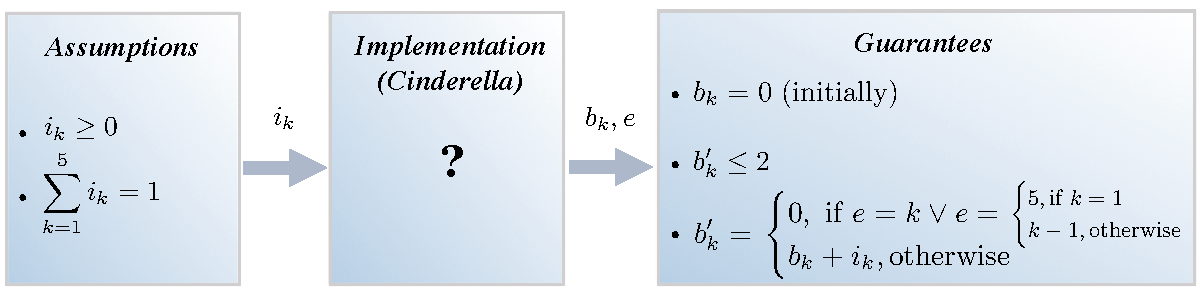
\includegraphics[scale=0.6]{agcontract.pdf}
\caption{An Assume-Guarantee contract.}
\label{fg:agcontract}
\end{figure}

We represent the system requirements using an \textit{Assume-Guarantee
Contract}. The \emph{assumptions} of the contract restrict the possible inputs that the
environment can provide to the system, while the \emph{guarantees}
describe safe reactions of the system to the outside world.

A (conceptually) simple example is shown in Fig.~\ref{fg:agcontract}. The contract describes a possible set of requirements for a specific instance of the Cinderella-Stepmother game. % that we introduced in Sect.~\ref{sec:example}.
Our goal is to synthesize an implementation that describes Cinderella's winning region of the game. Cinderella in this case is the implementation, as shown by the middle box in Fig.~\ref{fg:agcontract}. Cinderella's inputs are five different values $i_k$, $1 \leq k \leq 5$, determined by a random distribution of one unit of water by the Stepmother. During each of her turns Cinderella has to make a choice denoted by the output variable $e$, such that the buckets $b_k$ do not overflow during the next action of her Stepmother. We define the contract using the set of assumptions $A$ (left box in Fig.~\ref{fg:agcontract}) and the guarantee constraints $G$ (right box in Fig.~\ref{fg:agcontract}). For the particular example, it is possible to construct at least one implementation that satisfies $G$ given $A$ which is described in Sect.~\ref{sec:algexample}.
The proof of existence of such an implementation is the main concept behind the \emph{realizability} problem, while the automated construction of a witness implementation is the main focus of \emph{program synthesis}.

Given a proof of realizability of the contract in Fig.~\ref{fg:agcontract}, we are seeking for an efficient synthesis procedure that could provide an implementation. On the other hand, consider a variation of the example, where $A = \mathit{true}$. This is a practical case of an \emph{unrealizable} contract, as there is no feasible Cinderella implementation that can correctly react to Stepmother's actions. An example counterexample allows the Stepmother to pour random amounts of water into the buckets, leading to overflow of at least one bucket during each of her turns.

\section{Background}
\label{sec:background}
%\label{sec:formals}
We use two disjoint sets, $state$ and $inputs$, to describe a system.
A straightforward and intuitive way to represent an \emph{implementation} is by
defining a \emph{transition system}, composed of an initial state
predicate $I(s)$ of type $state \to bool$, as well as a transition relation
$T(s,i,s')$ of type $state \to inputs \to state \to bool$.

Combining the above, we represent an Assume-Guarantee (AG) contract using a set
of \emph{assumptions}, $A: state \rightarrow inputs \rightarrow bool$,
and a set of \emph{guarantees} $G$. The latter is further decomposed into two
distinct subsets $G_I: state \rightarrow bool$ and $G_T: state \rightarrow
inputs \rightarrow state \rightarrow bool$. The $G_I$ defines the set of valid
initial states, and $G_T$ contains constraints that need to be satisfied in
every transition between two states. Importantly, we
do not make any distinction between the internal state variables and the output variables in the
formalism. This allows us to use the state variables to (in some cases)
simplify the specification of guarantees since a contract
might not be always defined over all variables in the transition system.

Consequently, we can formally define a realizable contract, as one for which any
preceding state $s$ can  transition into a new state $s'$ that satisfies
the guarantees, assuming valid inputs. For a system to be ever-reactive, these
new states $s'$ should be further usable as preceding states in a future
transition. States like $s$ and $s'$ are called \textit{viable} if
and only if:
\begin{align}
\begin{split}
  \viable(s) &=
  \forall i. (A(s, i) \Rightarrow \exists s'.~ G_T(s, i,s')
\land \viable(s'))
\label{eq:viable}
\end{split}
\end{align}
This equation is recursive and we interpret it coinductively, i.e., as a
greatest fixpoint.
A necessary condition, finally, is that the intersection of sets of viable states
and initial states is non-empty. As such, to conclude that a contract
is realizable, we require that
\begin{equation}
\exists s. G_I(s) \land \viable(s)
\label{eq:nonempty}
\end{equation}

\noindent The synthesis problem is therefore to determine an initial state $s_i$ and function $f(s, i)$ such that $G_I(s_i)$ and $\forall s, i . \viable(s) \Rightarrow \viable(f(s, i))$.

\iffalse
The intuition behind our proposed algorithm in this paper relies on the
discovery of a fixpoint $F$ that only contains viable states.  We can determine whether $F$ is a fixpoint by proving the validity of the following formula:
\[
\forall s,i. \ (F(s) \land A(s,i) \Rightarrow \exists s'.G_{T}(s,i,s') \land F(s'))
\]

\noindent In the case where the greatest fixpoint $F$ is non-empty, we check whether it satisfies $G_{I}$ for some initial state.  If so, we proceed by extracting a witnessing initial state and witnessing skolem function $f(s, i)$ to determine $s'$ that is, by construction, guaranteed to satisfy the specification.

To achieve both the fixpoint generation and the witness extraction, we depend on \aeval, a solver for $\forall\exists$-formulas.

\subsection{Skolem functions and regions of validity}
\label{sec:aeval}


%\andreas{I believe the section can be a bit longer. I also think that the keyphrase ``region of validity'' needs to stand out more. Finally, a proof for Lemma 1, or at least an outline of it would be greatly appreciated.}

We rely on the already established algorithm to decide the validity of $\forall\exists$-formulas and extract Skolem functions, called \aeval~\cite{fedyukovich2015automated}.
It takes as input a formula $\forall x \,.\, \exists y  \,.\, \Phi (x, y)$ where $\Phi (x, y)$ is quantifier-free.
To decide its validity, \aeval first normalizes $\Phi (x, y)$ to the form $S(x) \Rightarrow T(x, y)$ and then attempts to extend all models of $S(x)$ to models of $T(x,y)$.
If such an extension is possible, then the input formula is valid, and a relationship between $x$ and $y$ are gathered in a Skolem function.
Otherwise the formula is invalid, and no Skolem function exists.
We refer the reader to~\cite{KatisFGBGW16} for more details on the Skolem-function generation.

Our approach presented in this paper relies on the fact that during each run, \aeval iteratively creates a set of formulas $\{P_i(x)\}$, such that each $P_i(x)$ has a common model with $S(x)$ and $P_i(x) \Rightarrow \exists y \,.\,T (x,y)$.
After $n$ iterations, \aeval establishes a formula $R_n(x) \eqdef \bigvee_{i=1}^n P_i(x)$ which by construction implies $\exists y\,.\,T(x,y)$.
If additionally $S(x)\Rightarrow R_n(x)$, the input formula is valid, and the algorithm terminates.
%
Fig.~\ref{fg:aeval} shows a Venn diagram for an example of the opposite scenario: $R_2(x) = T_1(x) \lor T_2(x)$, but the input formula is invalid.
However, models of each $S(x) \land P_i(x)$ can still be extended to a model of $T(x, y)$.
%Models of $S(x) \land \neg{R_2(x)}$ cannot be extended to models of $T(x,y)$, thus no formula $T_3(x)$ exists, and \aeval terminates.
% \john {Because we are are already using $A$ and $G$ to represent meaningful formulas I suggest that we use different symbols here so it is not confusing. Especially because the symbols have different signatures in these locations.}

In general, if after $n$ iterations $S(x) \land T(x,y) \land \neg R_n(x)$ is unsatisfiable,
then \aeval terminates.
Note that the formula $\forall x.~ S(x) \land R_n(x) \Rightarrow \exists y .~T(x,y)$ is valid by construction at any iteration of the algorithm.
%Thus, a Skolem function can be generated for it.
%Intuitively, a Skolem function
%describes how $y$ is computed from $s$ in order to satisfy the
%previous formula.
%
We say that $R_n(x)$ is a \emph{region of validity}, and in this work, we are interested in the \emph{maximal} regions of validity, i.e., the ones produced by disjoining all $\{P_i(x)\}$ produced by \aeval before termination and by conjoining it with $S(x)$.
Throughout the paper, we assume that all regions of validity are maximal.
% \john{It is a bit strange how we alternate using formulas that have no free variables along with formulas whose free variables are meant to be implicitly existentially quantified. I think we should either stick with a notation or explicitly say that free variables are interpreted to be existentially quantified.}

% \begin{lemma}
% If formula $\forall x \,.\,  S(x) \Rightarrow \exists y . T(x,y)$ is invalid, and $R_n(x)$ is the region of validity, then there is no other formula $S(x)$ such that $S(x) \land R_n(x) \Rightarrow S(x)$ and $\forall x \,.\,  S(x) \Rightarrow \exists y . T(x,y)$.
% \label{lem:subset}
% \end{lemma}

% \begin{proof}
% Suppose that $S(x)$ exists.
% Then $S(x) \land \neg{R_n(x)} \land S(x)$ is satisfiable, and its models are not contained in $R_n(x)$.
% It contradicts our assumption that \aeval has terminated since otherwise it would proceed for generating $T_{n+1}(x)$ which in turn would enlarge the region of validity.
% \end{proof}

\begin{figure}[!t]
\centering
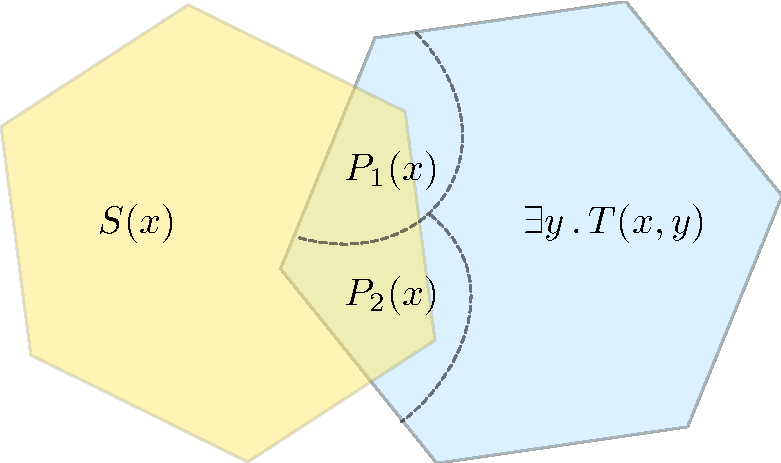
\includegraphics[scale=0.47]{aeval_invalid}
\caption{Region of validity computed for an example requiring \aeval to iterate two times.}
\label{fg:aeval}
\end{figure}

\begin{lemma}\label{lem:aeval}
  Let $R_n(x)$ be the region of validity returned by \aeval for  formula $\forall
  s.~ S(x) \Rightarrow \exists y\,.\,T(x,y)$. Then
%  \begin{equation*}
$  \forall x.~ S(x) \Rightarrow (R_n(x) \Leftrightarrow \exists y\,.\,T(x,y))$.
%  \end{equation*}
\end{lemma}
\begin{proof}
  ($\Rightarrow$) By construction of $R_n(x)$.

  ($\Leftarrow$) Suppose towards contradiction that the formula does
  not hold. Then there exists $x_0$ such that $S(x_0) \land (\exists
  y. T(x_0, y)) \land \neg R_n(x_0)$ holds. But this is a direct
  contradiction for the termination condition for \aeval. Therefore
  the original formula does hold.
\end{proof}

% \begin{corollary}
% If formula $\forall x \,.\,  S(x) \Rightarrow \exists y . T(x,y)$ is invalid, and $R_n(x)$ is the region of validity, then $S(x) \land R_n(x) \Leftrightarrow \exists y . T(x,y)$.
% \label{cor:intermediate}
% \end{corollary}

% \begin{proof}
% ($\Rightarrow$) is immediate from the definition of region of validity.
% ($\Leftarrow$).  Suppose towards contradiction that $s$ satisfies $\exists y . T(x,y)$ but not $S(x) \land R_n(x)$.  If we define $S = s$, we violate Lemma~\ref{lem:subset}.
% \end{proof} 

% \begin{corollary}
% If formula $\forall x \,.\,  S(x) \Rightarrow \exists y . T(x,y)$ is invalid, and $S(x) \land R_n(x)$ is the region of validity, then 
%  $\forall x \,.\, R_n(x) \Leftrightarrow (S(x) \Rightarrow \exists y . T(x,y))$ 
% \label{cor:subset}
% \end{corollary}

% \begin{proof}
% ($\Rightarrow$) Given $s$, suppose $R_n(x)$ is true.  If $S(x)$ is false, then by Corollary~\ref{cor:intermediate},  $\exists y . T(x,y)$ is false, so the implication holds.  Simlarly for $S(x)$ true.
% ($\Leftarrow$) Suppose $S(x) \Rightarrow \exists y . T(x,y)$ is true.  Suppose $S(x)$ is false.  Then $G(s, y)$ might be true and $R_n(x)$ might be false, violating our equivalence.  Boo!
% \end{proof}


\fi
\section{Synthesis from K-Inductive Proofs of Realizability}
\label{sec:kinductionsynth}
In this section we %define Assume-Guarantee contracts (Sect.~\ref{sec:pre}),
 sketch an existing algorithm for determining contract realizability
(Sect.~\ref{sec:old}), present our new algorithm that bridges the gap between the realizability checking and synthesis (Sect.~\ref{sec:realizability-synthesis}),
and finally illustrate how the algorithm works on an example
(Sect.~\ref{sec:example}).

\iffalse
\subsection{Assume-Guarantee Contracts}
\label{sec:pre}

One popular way to describe software requirements is through Assume-Guarantee
contracts, where requirements are expressed using safety properties that are
split into two categories, \emph{assumptions} and \emph{guarantees}.
Contract \emph{assumptions} are properties that restrict the set of valid inputs
a system can process, while \emph{guarantees} dictate system behavior by constraining system outputs.

For example, consider the contract with the assumption $A = \{x\neq
y\}$ and the guarantee $G = \{x \leq y \Longrightarrow z =
\textit{true}, x \geq y \Longrightarrow z = \textit{false}\}$, for a component with two inputs $x$ and $y$ and one output $z$.  By assumption, $x \neq y$, so the implemented system could set $z$ to true if $x < y$ and false otherwise. Of course, multiple implementations may exist for the same contract. An
alternative approach, for example, could set $z$ to false if $x > y$, and true
otherwise. Determining whether an implementation can be constructed to satisfy
the contract for all possible input sequences is the \emph{realizability} problem, while automatically constructing a witness of the proof of realizability of the contract is the \emph{program synthesis} problem.  The contract $(A,G)$ above is obviously \emph{realizable}, and therefore an implementation can be constructed.
However, if the assumption is omitted then the contract is \emph{unrealizable}, since there is no correct value for $z$ when $x=y$.

We describe a system using the disjoint sets $state$ and $inputs$.
Formally, an \emph{implementation} is a \emph{transition system}
described by an initial state predicate $I(s)$ of type $state \to
bool$ and by a transition relation $T(s,i,s')$ of type $state \to
inputs \to state \to bool$.

An Assume-Guarantee (AG) contract can be formally defined by a set of
\emph{assumptions} and a set of \emph{guarantees}. The
\emph{assumptions}, $A: state \rightarrow inputs \rightarrow bool$,
impose constraints over the inputs which may be modal in terms of the
previous state. The \emph{guarantees} $G$ consist of two separate
subsets $G_I: state \rightarrow bool$ and $G_T: state \rightarrow
inputs \rightarrow state \rightarrow bool$, where $G_I$ defines the
set of valid initial states, and $G_T$ specifies the properties that
need to be met during each new transition between two states. Note
that we do not necessarily expect that a contract would be defined
over all variables in the transition system, but we do not make any
distinction between internal state variables and outputs in the
formalism. This way, we can use state variables to (in some cases)
simplify the specification of guarantees.
\fi
%\vspace{-.5em}
\subsection{Realizability of Contracts}
\label{sec:old}
%\vspace{-.5em}

The synthesis algorithm proposed in this paper is built on top of our previous work on a realizability checking algorithm~\cite{gacek2015towards}. The coinductive notion of viable states described in Def.~\ref{eq:viable} is not useful to determine realizability in practice, and as such we have to use an approximation. With that in mind, we express the problem of realizability using the description of a state being \emph{extendable after n steps}, if any valid path of length $n-1$ starting from $s$ can be extended in response to any valid input:

%\begin{definition*}
%\label{def:extend}
%A state $s$ is extendable after $n$ steps, denoted $\mathit{Extend}_{n}(s)$, if
%any valid path of length $n-1$ starting from $s$ can be extended in response to
%any valid input.%
%
%\begin{equation}
\begin{multline}%
%\mathit{Extend}_{n}(s)
\extendable \triangleq \forall i_1, s_1, \ldots, i_n, s_n.\\ A(s, i_1) \land G_T(s, i_1, s_1)
\land \cdots \land
A(s_{n-1}, i_n) \land G_T(s_{n-1}, i_n, s_n)
\implies \\
\forall i.~ A(s_n, i) \implies \exists s'.~ G_T(s_n, i, s')
\label{def:extend}
\end{multline}
%\end{definition*}
%\end{equation}

The algorithm for realizability uses Def.~\ref{def:extend} in two
separate checks that correspond to the two traditional cases exercised
in k-induction. Initially, it is proved that the set of initial states is
not empty, by checking for the existence of at least one
state that satisfies $G_I$. For $\basecheck(n)$, we ensure
that all initial states are extendable for any path of length $k < n$,
while the inductive step of $\extendcheck(n)$ tries to prove that
all valid states are extendable for any path of length $n$. Therefore,
we attempt to find the smallest $n$, for which the two following
$\forall\exists$-formulas are valid:%
%
\begin{equation}
\label{eq:sbcheck}
\basecheck(n) \triangleq \forall k < n. (\forall s. G_I(s)
	  	\implies \extendablek)
\end{equation}%
%
\begin{equation}
\label{eq:echeck}
\extendcheck(n) \triangleq \forall s. \extendable
\end{equation}

The realizability checking algorithm has been used to effectively find cases
where the traditional consistency check (i.e. the existence of an assignment
to the input variables for which the output variables satisfy the contract)
failed to detect conflicts between stated requirements in case studies of
different complexity and importance. It has also been formally verified using the Coq proof assistant in terms of its
soundness, for the cases where it reports that a contract is
realizable~\cite{katis2015machine}.

\subsection{Program Synthesis from Proofs of Realizability}
\label{sec:realizability-synthesis}

%While the implemented algorithm on realizability provided us with meaningful
%results during the verification of several contracts,
%The main contribution of the paper is an algorithm for deriving implementations from the proof of a contract's realizability.
%Indeed, t
The algorithm sketched in Sect.~\ref{sec:old} can be further used for solving the more complex problem of
\emph{program synthesis} to automatically derive an implementation from the proof of a contract's realizability. 
%That is, we can automatically
%derive implementations from the proof of a contract's realizability.
%The limited power of SMT solvers
%in terms of solving formulas containing nested quantifiers immediately ruled
%out the prospect of using one as our primary synthesis tool. Fortunately,
%we are able to exploit our prior results in the scope of solving validity and
%Skolemizing $\forall\exists$-formulas (to be described in Sect.~\ref{sec:aeval}).
%The idea is simple.
Consider checks~\eqref{eq:sbcheck}
and~\eqref{eq:echeck} that are used in the realizability checking
algorithm. Both checks require that the reachable states explored are
extendable using Def.~\ref{def:extend}. The key insights are then 1)
we can start with a arbitrary state in $G_I$ since it is non-empty, 2)
we can use witnesses from the proofs of $\extendablek$ in
$\basecheck(n)$ to create a valid path of length $n-1$, and 3) we
can extend that path to arbitrary length by repeatedly using the
witness of the proof of $\extendable$ in
$\extendcheck(n)$.

In first order logic, witnesses for valid $\forall\exists$-formulas
are represented by Skolem functions. Intuitively, a Skolem function
expresses a connection between all universally quantified variables in
the left-hand side of the $\forall\exists$-formulas~\eqref{eq:sbcheck}
and~\eqref{eq:echeck} and the existentially quantified variable $s'$
within $\extendable$ \andreas{changed from ``$\mathit{Extend}$''} on the right-hand side. We generate Skolem functions from the validity of~\eqref{eq:sbcheck} and~\eqref{eq:echeck} using the \aeval tool~\cite{fedyukovich2015automated}. We refer the reader to Sect.~\ref{sec:aeval} for a brief description of its functionality.\andreas{We need to discuss whether we will have a dedicated \aeval section in the journal, as the space is quite limited.}

%Our algorithm uses the \aeval tool, detailed in Sect.~\ref{sec:aeval} \andreas{we need to discuss whether a dedicated section on \aeval is necessary for this paper, as the space is limited}
%, to generate such Skolem functions from the validity of~\eqref{eq:sbcheck} and~\eqref{eq:echeck}.

%\synthesisalgorithm

%% During the k-induction algorithm, two parallel
%% engines (\textsc{BaseEngine, ExtendEngine}) handle the base and
%% inductive step checks of validity of $\forall\exists$-formulas.
%% The proof of a formula's validity is closely tied to the process of
%% Skolemization: for every step that \textit{BaseCheck(n)} is valid,
%% \aeval provides a Skolem function to witness that validity.


\begin{figure}
\scalebox{.85}{
\begin{minipage}{0.65\textwidth}
\begin{algorithm}[H]
\caption{\jsyn (A : assumptions, G : guarantees)}
\label{alg:kindsynthesis}
\begin{algorithmic}[1]
	\State $Skolems \gets \langle \rangle$;%\Comment{List of Skolem Functions}
	\State $InitResult \gets $\textsc{Sat?}$(G_I)$;
	\If{$(\isUnsat(InitResult))$}
		\Return \unrealizable, $\emptyset$, $\langle \rangle$;
	\EndIf
	\For{$(i \gets 0; \mathbf{true}; i \gets i + 1)$}
		\State $\tuple{\mathit{valid}, \skolems} \gets \aeval(\extendcheck(i))$
%		\State $ExtendResult \gets \aeval(ExtendCheck(i))$;
		%\If{$(\isValid(ExtendResult))$}
		\If{$\mathit{valid}$}
			\State $Skolems.Add(\skolems)$
			%\State $Skolems.Add(ExtendResult.Skolem)$;
			\Return \realizable, $Skolems$;
		\EndIf
		\State $\tuple{\mathit{valid}, \skolems} \gets \aeval(\basecheck_{k}(i))$
		%\State $BaseResult \gets \textsc{\aeval}(BaseCheck_{k}(i))$;
		%\If{$(\isInvalid(BaseResult))$}
		\If{$\lnot \mathit{valid}$}
			\Return \unrealizable, $\emptyset$, $\langle \rangle$;
		\EndIf
		\State $Skolems.Add(\skolems)$
		%\State $Skolems.Add(BaseResult.Skolem)$;
	\EndFor
\end{algorithmic}
\end{algorithm}
\end{minipage}
}
\hspace{1cm}
\scalebox{.8}{
\begin{minipage}{0.38\textwidth}
\setcounter{algorithm}{0}
\begin{template}[H]
\caption{Structure of an implementation}
\label{alg:synt}
\begin{algorithmic}[1]
	\State $\textsc{assign\_Init()}$;
	\State $\textsc{read\_inputs()}$; 		
	\State $\textsc{Skolems}[0]()$;
  	\State $\ldots$
  	\State $\textsc{read\_inputs()}$;
  	\State $\textsc{Skolems}[k-1]()$;
	\While{true}
 		\State $\textsc{read\_inputs()}$;
 		\State $\textsc{Skolems}[k]()$;
 		\State $\textsc{update\_history()}$;
	\EndWhile
\end{algorithmic}
\end{template}
\end{minipage}
}
\end{figure}

Alg.~\ref{alg:kindsynthesis} named \jsyn provides a summary of the synthesis
procedure. The algorithm first determines whether the set of initial states $G_I$ is non-empty.
Second, it attempts to construct an inductive proof of the system's
realizability, using \aeval\ to find Skolem witnesses. For each call of \aeval we write $\tuple{x, y} \gets \aeval(\ldots)$: $x$ specifies if the given formula is valid or not, and $y$ contains the Skolem function (only in case of the validity). The algorithm iteratively proves $\mathit{BaseCheck_k(i)} \triangleq \forall s. G_I(s) \implies \mathit{Extend}_i(s)$ and accumulates the resulting Skolem functions. If $\mathit{BaseCheck_k(i)}$ ever fails, we know $\mathit{BaseCheck(i)}$ would also fail and so the system is unrealizable. At the same time, the algorithm tries to prove $\mathit{ExtendCheck(i)}$. As soon as the inductive step of $\mathit{ExtendCheck(i)}$ passes, we have a complete k-inductive proof stating that the contract is realizable. We then complete our synthesis procedure by generating a Skolem function that
corresponds to the inductive step, and return the list of the Skolem functions.  Note that in Alg.~\ref{alg:kindsynthesis} for a particular depth $k$, we perform the extends check prior to the base check. The intuition is that $\mathit{BaseCheck(i)}$ checks $\forall k < i$; thus, it is one step ``smaller'' than the extends check and this avoids a special case at $k=0$.

Given a list of Skolem functions, it remains to plug them into
an implementation skeleton as shown in Template~\ref{alg:synt}.
The combination of Lustre models and k-inductive proofs
allow the properties in the model to manipulate the
 values of variables up to $k-1$ steps in the past. Thus,
the first step of an implementation  (method \textsc{assign\_Init()})
 creates an array for each state variable of size $k+1$, where
$k$ is the depth of the solution to Alg.~\ref{alg:kindsynthesis}.
This array represents the depth of history necessary to compute
the recurrent Skolem function produced by the $\extendcheck(n)$ process.
The $\basecheck(n)$ Skolem functions initialize this history.

In each array, the $i$-th element, with $0\leq i \leq k-1$,
corresponds to the value assigned to the variable after the call to
$i$-th Skolem function. As such, the first $k-1$ elements of each array
correspond to the $k-1$ Skolem functions produced by the
$\basecheck(n)$ process, while the last element is used by the
Skolem function generated from the formula corresponding to the
$\extendcheck(n)$ process.

The template uses the Skolem functions generated by \aeval for each
of the $\basecheck(n)$ instances to describe the initial behavior of
the implementation prior to depth $k$.  %\textcolor{red}{This process starts
% from the memory-free witness $\init$ to the initial guarantee $G_I$, which is
%assigned in method \textsc{assign\_Init()}}.
There are two ``helper'' operations:
\textsc{update\_history()} shifts each element in the arrays one position
forward (the 0-th value is simply forgotten), and \textsc{read\_inputs()} reads the
current values of inputs into the $i$-th element of the variable arrays,
where $i$ represents the $i$-th step of the process.
Once the history is entirely initialized using the $\basecheck(n)$ Skolem functions,
we add the Skolem function for the $\extendcheck(n)$ instance to describe the
recurrent behavior of the implementation (i.e., the next value of outputs in
each iteration in the infinite loop).

To establish the correctness of the algorithm,
we have constructed machine-checked proofs as to the validity of $\mathit{BaseCheck(n)}$ and
$\mathit{ExtendCheck(n)}$ using the Skolem functions.
The entirety of the models explored in
this paper only involved proofs of realizability of length $k$ equal to 0 or
1.
As such, we limited our proofs of soundness to these two specific cases. We will
extend the proofs to capture any arbitrary $k$ as part of our future work.
The theorems were written and proved using the Coq proof
assistant.~\footnote{The proofs can be found
at~\href{https://github.com/andrewkatis/Coq}{https://github.com/andrewkatis/Coq}}.

\begin{theorem}[Bounded Soundness of BaseCheck and ExtendCheck using Skolem Functions]
Let $\basecheck_{S(s_n,i,s')}(n)$ and $\extendcheck_{S(s_n,i,s')}(n)$, $n \in {0,1}$, be the valid variations of the corresponding formulas $\mathit{BaseCheck(n)}$ and $\mathit{ExtendCheck(n)}$, where the existentially quantified part $\exists s'.~G_T(s_n, i, s')$ has been substituted with a witnessing Skolem function
$S(s_n,i,s')$.  We have that:
\begin{itemize}
\item $\forall (A,G_{I},G_{T}). \mathit{BaseCheck}(n) \Rightarrow \mathit{BaseCheck}_{S(s_n,i,s')}(n)$
\item $\forall (A,G_{I},G_{T}). \mathit{ExtendCheck}(n) \Rightarrow
ExtendCheck_{S(s_n,i,s')}(n)$
\end{itemize}
\end{theorem}
\begin{proof}
The proof uses the definition $\mathit{Extend}_n(s)$ of an extendable state,
after replacing the next-step states with corresponding Skolem functions. From there,
the proof of the two implications is straightforward.
\qed
\end{proof}

\subsection{\jsyn and the issue of soundness on ``unrealizable'' results}

While we were able to use \jsyn to synthesize implementations for a significant number of complex contracts, the algorithm faces a fundamental problem when it comes to the soundness of ``unrealizable'' results, where it might declare a given contract as being non-implementable, while an implementation does exist. The Cinderella-Stepmother, introduced in Section~\ref{sec:example} helps us demonstrate this in a meaningful way.

\begin{figure}[!t]
\centering
 \begin{Verbatim}[fontsize=\scriptsize]
const C = 2.0;

-- empty buckets e and e+1 each round
node game(i1,i2,i3,i4,i5: real; e: int) returns (guarantee: bool);
var
  b1, b2, b3, b4, b5 : real;
let
  assert i1 >= 0.0 and i2 >= 0.0 and i3 >= 0.0 and i4 >= 0.0 and i5 >= 0.0;
  assert i1 + i2 + i3 + i4 + i5 = 1.0;

  b1 = 0.0 -> (if (e = 5 or e = 1) then i1 else (pre(b1) + i1));
  b2 = 0.0 -> (if (e = 1 or e = 2) then i2 else (pre(b2) + i2));
  b3 = 0.0 -> (if (e = 2 or e = 3) then i3 else (pre(b3) + i3));
  b4 = 0.0 -> (if (e = 3 or e = 4) then i4 else (pre(b4) + i4));
  b5 = 0.0 -> (if (e = 4 or e = 5) then i5 else (pre(b5) + i5));

  guarantee = b1 <= C and b2 <= C and b3 <= C and b4 <= C and b5 <= C;

  --%REALIZABLE i1, i2, i3, i4, i5;
  --%PROPERTY guarantee;
tel;
 \end{Verbatim}
\vspace{-1em}
\caption{An Assume-Guarantee contract for the Cinderella-Stepmother game in Lustre.}

\label{fg:cind}
\end{figure}

Fig.~\ref{fg:cind} shows one possible interpretation of the contract designed
for the instance of the Cinderella-Stepmother game in Fig.~\ref{fg:agcontract}. The contract
is expressed in Lustre~\cite{lustrev6}, a language
that has been extensively used for specification as well as implementation of
safety-critical systems, and is the kernel language in SCADE, a popular tool in
model-based development. The contract is defined as a Lustre node \texttt{game}, with a global
constant \texttt{C} denoting the bucket capacity. The node describes the game itself,
through the problem's input and output variables. The main input is Stepmother's
distribution of one unit of water over five different input variables,
\texttt{i1} to \texttt{i5}. While the node contains a sixth input argument,
namely \texttt{e}, this is in fact used as the output of the system that we want to
implement, representing Cinderella's choice at each of her turns.

We specify the system's inputs \texttt{i1}, \ldots, \texttt{i5} using the \texttt{REALIZABLE} statement and define the contract's assumptions over them: $A(i_1, \ldots, i_5) = (\bigwedge_{k=1}^{5} i_k >= 0.0) \land (\sum_{k=1}^{5} i_{k} = 1.0)$. The assignment to boolean variable \texttt{guarantee} (distinguished via the \texttt{PROPERTY} statement) imposes the guarantee constraints on the buckets' states through the entire
duration of the game, using the local variables \texttt{b1} to \texttt{b5}.
Initially, each bucket is empty, and with each transition to a new state, the contents depend on
whether Cinderella chose the specific bucket, or an adjacent one. If so, the value of each \texttt{b}$_k$ at the the next turn becomes equal to the value of the corresponding input variable \texttt{i}$_k$. Formally, for the initial state, $G_{I}(C, b_1, \ldots, b_5) = (\bigwedge_{k=1}^{5} b_k = 0.0) \land (\bigwedge_{k = 1}^{5} b_k \le C)$, while the transitional guarantee is $G_T([C,b_1, \ldots, b_5, e], i_1, \ldots, i_5, [C',b_{1}', \ldots, b_{5}',e']) = (\bigwedge_{k=1}^{5} b_{k}' = ite(e = k \lor e = k_{prev}, i_k, b_k + i_k) \land (\bigwedge_{k=1}^{5} b_{k}' \le C')$, where $k_{prev} = 5$ if $k = 1$, and $k_{prev} = k - 1$ otherwise. Interestingly, the lack of explicit constraints over $e$, i.e. Cinderella's choice, permits the action of Cinderella skipping her current turn, i.e. she does not choose to empty any of the buckets. With the addition of the guarantee $(e = 1) \lor \ldots \lor (e =5)$, the contract is still realizable, and the implementation is verifiable, but Cinderella is not allowed to skip her turn anymore.

If the bucket was not covered by Cinderella's choice, then its contents are
updated by adding Stepmother's distribution to the volume of water that the
bucket already had. The arrow (\texttt{->}) operator distinguishes the initial state (on the left) from subsequent states (on the right), and variable values in the previous state can be accessed using the \texttt{pre} operator.
The contract should only be realizable if, assuming valid inputs given by the Stepmother
(i.e. positive values to input variables that add up to one water unit),
Cinderella can keep reacting indefinitely, by providing outputs that satisfy the
guarantees (i.e. she empties buckets in order to prevent overflow in Stepmother's next turn).


\begin{figure}[!t]
\centering
 \begin{Verbatim}[fontsize=\scriptsize]
	 ++++++++++++++++++++++++++++++++++++++++++++++++++++++++++
	      UNREALIZABLE || K = 6 || Time = 2.017s
	                 Step
	      variable      0    1      2      3      4      5
	      INPUTS
	      i1            0    0      0 0.416* 0.944* 0.666*
	      i2            1    0 0.083* 0.083*      0 0.055*
	      i3            0    1 0.305*    0.5 0.027* 0.194*
	      i4            0    0 0.611*      0      0 0.027*
	      i5            0    0      0      0 0.027* 0.055*
	
	      OUTPUTS
	      e             1    3      1      5      4      5
	
	      NODE OUTPUTS
	      guarantee   true true   true   true   true  false
	
	      NODE LOCALS
	      b1            0    0      0 0.416* 1.361* 0.666*
	      b2            0    0 0.083* 0.166* 0.166* 0.222*
	      b3            0    1 1.305* 1.805* 1.833* 2.027*
	      b4            0    0 0.611* 0.611*      0 0.027*
	      b5            0    0      0      0 0.027* 0.055*
	
	      * display value has been truncated
	 ++++++++++++++++++++++++++++++++++++++++++++++++++++++++++
 \end{Verbatim}
\vspace{-1.5em}
\caption{Spurious counterexample for Cinderella-Stepmother example using \jsyn}
\label{fg:cex}
\end{figure}

Applying \jsyn to the contract that we described provides us with a pessimistic answer. \jsyn determines that the contract is unrealizable, and provides the counterexample shown in Fig.~\ref{fg:cex} as its witness. Nevertheless, this spurious counterexample perfectly depicts the issue, as the underlying SMT solver is incapable of choosing the correct
buckets to empty, leading eventually to a state where an overflow occurs for the third bucket. This comes in contrast with the established fact from related literature that a winning strategy exists for Cinderella, as long as the bucket capacity \texttt{C} is between 1.5 and 3~\cite{bodlaender2012cinderella}.

\iffalse
\subsection{An Illustrative Example}
%\label{sec:example}

\begin{figure}[t!]
\centering
\begin{minipage}[c]{0.6\textwidth}
\begin{Verbatim}[fontsize=\scriptsize]
node top(x : int; state: int) returns (  );
var
  bias : int;
  guarantee1, guarantee2, guarantee3,
  guarantee4, guarantee5, guarantee_all : bool;
  bias_max : bool;
let
  bias = 0 -> (if x = 1 then 1 else -1) + pre(bias);
  bias_max = false ->
	(bias >= 2 or bias <= -2) or pre(bias_max);
  assert (x = 0) or (x = 1);
  guarantee1 = (state = 0 => (bias = 0));
  guarantee2 = true ->
  	(pre(state = 0) and x = 1) => state = 2;
  guarantee3 = true ->
  	(pre(state = 0) and x = 0) => state = 1;
  guarantee4 = bias_max => state = 3;
  guarantee5 = state = 0 or state = 1
                    or state = 2 or state = 3;
  guarantee_all = guarantee1 and guarantee2 and
          guarantee3 and guarantee4 and guarantee5;
  --%PROPERTY guarantee_all;
  --%REALIZABLE x;
tel;
 \end{Verbatim}
\end{minipage}
\scalebox{.7}{
\begin{minipage}[H]{0.5\textwidth}
\centering
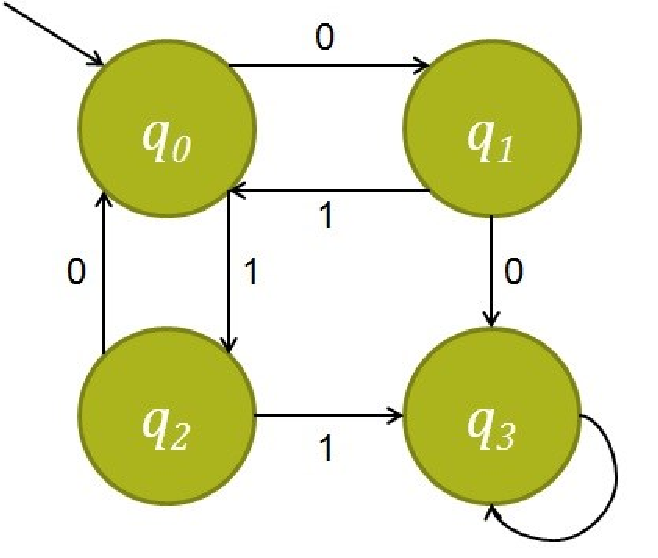
\includegraphics[width=\textwidth,height=0.8\textheight,keepaspectratio]{example-crop}
\end{minipage}}
%\vspace{-0.5em}
\caption{Requirements and possible implementation for example}
%\vspace{-1.5em}
\label{fg:example}
\end{figure}

The left side of Fig.~\ref{fg:example} shows a (somewhat contrived) contract for a system that detects whether a string of two zeros or two ones ever occurs in a stream of inputs written in a dialect of the Lustre language~\cite{lustrev6}.  The right side shows a possible implementation of that contract, visualized as a state machine.
%
Rather than use this implementation, we would like to synthesize a new one directly from the contract. There are two unassigned variables in the contract,
\texttt{x} and \texttt{state}.
The \texttt{{-}{-}\%REALIZABLE} statement specifies that \texttt{x} is a system
input, and by its absence, that \texttt{state} is a system output. The contract's 
assumption is specified by the \texttt{assert} statement and restricts the allowable input values of \texttt{x} to either 0 or 1. We also have five guarantees:
\texttt{guarantee2} and \texttt{guarantee3} are used to indirectly
describe some possible transitions in the automaton;\footnote{In Lustre, the
arrow (\texttt{->}) and \texttt{pre} operators are used to provide an initial value and access the previous value of a stream, respectively.} \texttt{guarantee5} specifies the range of
values of variable \texttt{state};
\texttt{guarantee1} and \texttt{guarantee4} are the requirements with respect to
two local variables, \texttt{bias} and \texttt{bias\char`_max}, where
 \texttt{bias} calculates the number of successive ones or
zeros read by the automaton and \texttt{bias\char`_max} indicates that at least two zeros or two ones have been read in a row.

Note that while Lustre is a compilable language, using standard compilation tools the ``program'' in Fig.~\ref{fg:example} would not compile into a meaningful implementation: it has no outputs!  Instead, it defines the guarantees we wish to enforce within the controller, and our synthesis tool will construct a program which meets the guarantees.

The realizability check on this example succeeds with a k-inductive
proof of length $k = 1$. The two corresponding
$\forall\exists$-formulas ($k=0$ for the base check and $k=1$ for the
inductive check) are valid, and thus \aeval extracts two witnessing
Skolem functions that effectively describe assignments to the local
variables of the specification, as well as to \texttt{state} (see
Appendix~\ref{app:ex} for the particular formulas).

The Skolem functions are used to construct the final implementation
following the outline provided in Template~\ref{alg:synt}.
The main idea is to redefine each variable in the model
as an array of size equal to $k$ and
to use the $k$-th element of each array as the corresponding output of the call
to $k$-th Skolem function. After this initialization process, we use an infinite
loop to assign new values to the element corresponding to the last Skolem
function, to cover the inductive step of the original proof. The final code, a
snippet of which is presented below, is 144 lines long.
Since each Skolem is represented by an $\mathit{ite}$-statement (to be explained
in Sect.~\ref{sec:aeval}), each branch is further encoded into a C-code, as
shown in Figure~\ref{fg:snippet}.

\begin{figure}[t!]
%\begin{framed}
\vspace{-2em}
\begin{minipage}{2.0\textwidth}
\begin{lstlisting}[basicstyle=\scriptsize,language=C]{Name=test2}
if (((x[1] == 1 && (-1 == bias[0])) || (x[1] == 0 && (1 == bias[0])))
     && !bias_max[0] && (state[0] != 0 || x[1] == 0)
     && (!state[0] != 0 || x[1] == 1)) {
  bias_max[1] = 0;
  bias[1] = 0;
  state[1] = 0;
}
\end{lstlisting}%
\end{minipage}
%\end{framed}
\vspace{-1em}
\caption{A code snippet of the synthesized implementation for the contract from Fig.~\ref{fg:example}.}
\vspace{-.5em}
\label{fg:snippet}
\end{figure}%

Notice how each variable is represented by an array in the snippet above.
We chose to use this easy to understand representation in order to effectively
store all the past $k-1$ values of each variable, that may be needed during the
construction of the k-inductive proof.

Recall that the user-defined model explicitly specifies only two transitions
(via \texttt{guarantee2} and \texttt{guarantee3}), while the set of implicitly defined transitions (via \texttt{guarantee1} and \texttt{guarantee4}) is incomplete.
%For example, the model does not specify an incoming transition to (\texttt{state = 0}).
Interestingly, our synthesized implementation turns all implicit transitions
into explicit ones which makes them executable and, furthermore, adds the
missing ones (e.g., as in the aforementioned snippet, from \texttt{state = 1} to \texttt{state = 0}).
\fi
\section{Validity-Guided Synthesis from Assume-Guarantee Contracts}
\label{sec:fixpointsynth}

The lack of soundness for unrealizable results in \jsyn was the catalyst towards pursuing a better approach. The intuition behind the second algorithm in this paper relies on the discovery of a fixpoint $F$ that only contains viable states.  We can determine whether $F$ is a fixpoint by proving the validity of the following formula:
\[
\forall s,i. \ (F(s) \land A(s,i) \Rightarrow \exists s'.G_{T}(s,i,s') \land F(s'))
\]

\noindent In the case where the greatest fixpoint $F$ is non-empty, we check whether it satisfies $G_{I}$ for some initial state.  If so, we proceed by extracting a witnessing initial state and witnessing skolem function $f(s, i)$ to determine $s'$ that is, by construction, guaranteed to satisfy the specification.

To achieve witness extraction, we again depend on \aeval, with its support for generating \textit{regions of validity} being particularly crucial for the computation of fixpoints.

\subsection{Skolem functions and regions of validity}
\label{sec:aeval}


%\andreas{I believe the section can be a bit longer. I also think that the keyphrase ``region of validity'' needs to stand out more. Finally, a proof for Lemma 1, or at least an outline of it would be greatly appreciated.}

We rely on the already established algorithm to decide the validity of $\forall\exists$-formulas and extract Skolem functions, called \aeval~\cite{fedyukovich2015automated}.
It takes as input a formula $\forall x \,.\, \exists y  \,.\, \Phi (x, y)$ where $\Phi (x, y)$ is quantifier-free.
To decide its validity, \aeval first normalizes $\Phi (x, y)$ to the form $S(x) \Rightarrow T(x, y)$ and then attempts to extend all models of $S(x)$ to models of $T(x,y)$.
If such an extension is possible, then the input formula is valid, and a relationship between $x$ and $y$ are gathered in a Skolem function.
Otherwise the formula is invalid, and no Skolem function exists.
We refer the reader to~\cite{KatisFGBGW16} for more details on the Skolem-function generation.

Our approach presented in this paper relies on the fact that during each run, \aeval iteratively creates a set of formulas $\{P_i(x)\}$, such that each $P_i(x)$ has a common model with $S(x)$ and $P_i(x) \Rightarrow \exists y \,.\,T (x,y)$.
After $n$ iterations, \aeval establishes a formula $R_n(x) \eqdef \bigvee_{i=1}^n P_i(x)$ which by construction implies $\exists y\,.\,T(x,y)$.
If additionally $S(x)\Rightarrow R_n(x)$, the input formula is valid, and the algorithm terminates.
%
Fig.~\ref{fg:aeval} shows a Venn diagram for an example of the opposite scenario: $R_2(x) = T_1(x) \lor T_2(x)$, but the input formula is invalid.
However, models of each $S(x) \land P_i(x)$ can still be extended to a model of $T(x, y)$.
%Models of $S(x) \land \neg{R_2(x)}$ cannot be extended to models of $T(x,y)$, thus no formula $T_3(x)$ exists, and \aeval terminates.
% \john {Because we are are already using $A$ and $G$ to represent meaningful formulas I suggest that we use different symbols here so it is not confusing. Especially because the symbols have different signatures in these locations.}

In general, if after $n$ iterations $S(x) \land T(x,y) \land \neg R_n(x)$ is unsatisfiable,
then \aeval terminates.
Note that the formula $\forall x.~ S(x) \land R_n(x) \Rightarrow \exists y .~T(x,y)$ is valid by construction at any iteration of the algorithm.
%Thus, a Skolem function can be generated for it.
%Intuitively, a Skolem function
%describes how $y$ is computed from $s$ in order to satisfy the
%previous formula.
%
We say that $R_n(x)$ is a \emph{region of validity}, and in this work, we are interested in the \emph{maximal} regions of validity, i.e., the ones produced by disjoining all $\{P_i(x)\}$ produced by \aeval before termination and by conjoining it with $S(x)$.
Throughout the paper, we assume that all regions of validity are maximal.
% \john{It is a bit strange how we alternate using formulas that have no free variables along with formulas whose free variables are meant to be implicitly existentially quantified. I think we should either stick with a notation or explicitly say that free variables are interpreted to be existentially quantified.}

% \begin{lemma}
% If formula $\forall x \,.\,  S(x) \Rightarrow \exists y . T(x,y)$ is invalid, and $R_n(x)$ is the region of validity, then there is no other formula $S(x)$ such that $S(x) \land R_n(x) \Rightarrow S(x)$ and $\forall x \,.\,  S(x) \Rightarrow \exists y . T(x,y)$.
% \label{lem:subset}
% \end{lemma}

% \begin{proof}
% Suppose that $S(x)$ exists.
% Then $S(x) \land \neg{R_n(x)} \land S(x)$ is satisfiable, and its models are not contained in $R_n(x)$.
% It contradicts our assumption that \aeval has terminated since otherwise it would proceed for generating $T_{n+1}(x)$ which in turn would enlarge the region of validity.
% \end{proof}

\begin{figure}[!t]
\centering
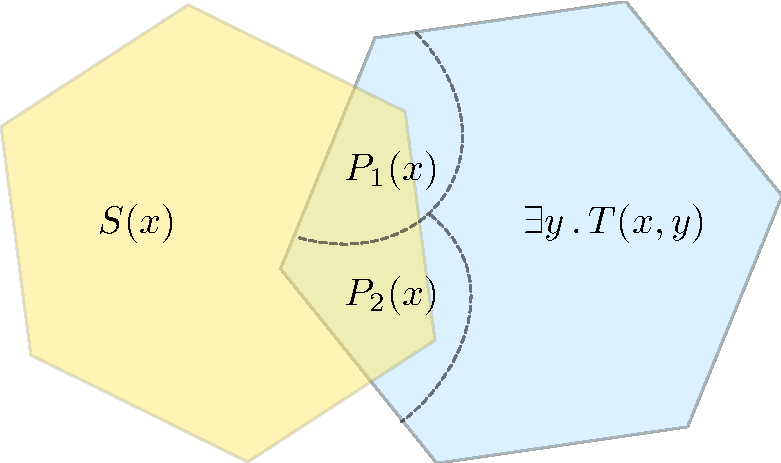
\includegraphics[scale=0.47]{aeval_invalid}
\caption{Region of validity computed for an example requiring \aeval to iterate two times.}
\label{fg:aeval}
\end{figure}

\begin{lemma}\label{lem:aeval}
  Let $R_n(x)$ be the region of validity returned by \aeval for  formula $\forall
  s.~ S(x) \Rightarrow \exists y\,.\,T(x,y)$. Then
%  \begin{equation*}
$  \forall x.~ S(x) \Rightarrow (R_n(x) \Leftrightarrow \exists y\,.\,T(x,y))$.
%  \end{equation*}
\end{lemma}
\begin{proof}
  ($\Rightarrow$) By construction of $R_n(x)$.

  ($\Leftarrow$) Suppose towards contradiction that the formula does
  not hold. Then there exists $x_0$ such that $S(x_0) \land (\exists
  y. T(x_0, y)) \land \neg R_n(x_0)$ holds. But this is a direct
  contradiction for the termination condition for \aeval. Therefore
  the original formula does hold.
\end{proof}

% \begin{corollary}
% If formula $\forall x \,.\,  S(x) \Rightarrow \exists y . T(x,y)$ is invalid, and $R_n(x)$ is the region of validity, then $S(x) \land R_n(x) \Leftrightarrow \exists y . T(x,y)$.
% \label{cor:intermediate}
% \end{corollary}

% \begin{proof}
% ($\Rightarrow$) is immediate from the definition of region of validity.
% ($\Leftarrow$).  Suppose towards contradiction that $s$ satisfies $\exists y . T(x,y)$ but not $S(x) \land R_n(x)$.  If we define $S = s$, we violate Lemma~\ref{lem:subset}.
% \end{proof} 

% \begin{corollary}
% If formula $\forall x \,.\,  S(x) \Rightarrow \exists y . T(x,y)$ is invalid, and $S(x) \land R_n(x)$ is the region of validity, then 
%  $\forall x \,.\, R_n(x) \Leftrightarrow (S(x) \Rightarrow \exists y . T(x,y))$ 
% \label{cor:subset}
% \end{corollary}

% \begin{proof}
% ($\Rightarrow$) Given $s$, suppose $R_n(x)$ is true.  If $S(x)$ is false, then by Corollary~\ref{cor:intermediate},  $\exists y . T(x,y)$ is false, so the implication holds.  Simlarly for $S(x)$ true.
% ($\Leftarrow$) Suppose $S(x) \Rightarrow \exists y . T(x,y)$ is true.  Suppose $S(x)$ is false.  Then $G(s, y)$ might be true and $R_n(x)$ might be false, violating our equivalence.  Boo!
% \end{proof}



\begin{algorithm*}[!t]
\caption{\jsynvg (A : assumptions, G : guarantees)}
\label{alg:synthesis}
\begin{algorithmic}[1]
	\State $F(s) \gets \mathit{true}$\label{alg:init};\Comment{Fixpoint of viable states}
	\While{$\mathit{true}$}
		\State $\phi \gets \forall s,i. \ (F(s) \land A(s,i) \Rightarrow \exists s'.G_{T}(s,i,s') \land F(s'))$\label{alg:ae1};
		\State $\tuple{\mathit{valid}, \subs, \skolems} \gets \aeval(\phi) \label{alg:val1}$;
		\If{$\mathit{valid}$\label{alg:val2}}
            \If{$\exists s . G_{I}(s) \land F(s)$}
				\Return $\tuple{\realizable, \skolems, s, F}$\label{alg:issat};
			\Else{\Comment{Empty set of initial or viable states}}
		 		\Return $\unrealizable$\label{alg:unreal};
		 	\EndIf
		\Else{\Comment{Extract region of validity $Q(s,i)$}}
			\State $Q(s,i) \gets \subs$\label{alg:valreg};
			\State $\phi' \gets \forall s. \ (F(s) \Rightarrow \exists i. A(s,i) \land \lnot
			Q(s,i))$\label{alg:ae2};
			\State $\tuple{\_, \mathit{violatingRegion}, \_} \gets \aeval(\phi')$;
			\State $W(s) \gets \mathit{violatingRegion}$;
			\State $F(s) \gets F(s) \land \lnot W(s)$\label{alg:rem};\Comment{Refine set of viable states}	
		\EndIf
	\EndWhile
\end{algorithmic}
\end{algorithm*}

Alg.~\ref{alg:synthesis}, named \jsynvg (for {\em validity guided}), shows the validity-guided technique that we use towards the automatic synthesis of implementations. The specification is written using the Assume-Guarantee convention that we described in Section~\ref{sec:background} and is provided as an input. For this algorithm we modify the form of the results provided by \aeval to $\tuple{x, y, z} \gets \aeval(\ldots)$: $x$ again specifies if the formula is (not) valid, $y$ identifies the region of validity (in both cases), and $z$ -- the Skolem function (only in case of the validity).

The algorithm maintains a formula $F(s)$ which is initially assigned $\mathit{true}$ (line~\ref{alg:init}).
It then attempts to strengthen $F(s)$ until it only contains viable states (recall Eqs.~\ref{eq:viable}
and~\ref{eq:nonempty}), i.e., a greatest fixpoint is reached.
We first encode Eq.~\ref{eq:viable} in a formula $\phi$ and then provide it as input to \aeval (line~\ref{alg:val1}) which determines its validity (line~\ref{alg:val2}).
If the formula is valid, then a witness $\skolems$ is non-empty.
By construction, it contains valid assignments to the existentially quantified variables of $\phi$.
In the context of viability, this witness is capable of providing viable states that can be used as a safe
reaction, given an input that satisfies the assumptions.

With the valid formula $\phi$ in hand, it remains to check that the fixpoint intersects with the initial states, i.e., to find a model of formula in Eq.~\ref{eq:nonempty} by a simple satisfiability check.
If a model exists, it is directly combined with the extracted witness and used towards an implementation of the system, and the algorithm terminates (line~\ref{alg:issat}).
Otherwise, the contract is unrealizable since either there are no states that satisfy the
initial state guarantees $G_I$, or the set of viable states $F$ is empty.


If $\phi$ is not true for every possible assignment of the universally
quantified variables, \aeval provides a \textit{region of validity} $Q(s,i)$
(line~\ref{alg:valreg}).
%an exact subset of $F(s) \land A(s,i)$, namely $Q(s,i)$, which, if plugged in
% the original left-hand side of $\phi$, makes the resulting formula valid. We will refer to such subsets as \textit{regions of
%validity}.
At this point, one might assume that $Q(s,i)$ is sufficient to restrict $F$ towards a solution. This is not the case since $Q(s,i)$ creates a subregion
involving both state and input variables. As such, it may contain constraints
over the contract's inputs above what are required by $A$, ultimately leading to implementations that only work correctly for a small part of the input domain.

Fortunately, we can again use \aeval's capability of providing regions of validity
towards removing inputs from $Q$.  Essentially, we want to remove those states from $Q$ if even one input causes them to violate the formula on line~\ref{alg:ae1}.  We denote by $W$ the {\em violating region} of $Q$.  To construct $W$, \aeval  determines
the validity of formula $\phi' \gets \forall s. \ (F(s) \Rightarrow \exists
i. A(s,i) \land \lnot Q(s,i))$ (line~\ref{alg:ae2}) and computes
a new region of validity.

If $\phi'$ is invalid, it indicates that there are still non-violating states (i.e., outside $W$) that may lead to a fixpoint.
Thus, the algorithm removes the unsafe states from $F(s)$ in line~\ref{alg:rem}, and iterates until a greatest fixpoint for $F(s)$ is reached.  %If the system is unrealizable, this fixpoint (which may be the formula `false') does not intersect the set of initial states.
If $\phi'$ is valid, then every state in $F(s)$ is unsafe, under a specific input that satisfies the contract assumptions (since $\lnot Q(s,i)$ holds in this case), and the specification is unrealizable (i.e., in the next iteration, the algorithm will reach line~\ref{alg:unreal}).


%or until $W(s)$ becomes valid, that is, for any assignment of the state variables $s$, we have an input that satisfies the assumptions and violates $Q$.  In this case, every state in $F$ has some failing input and the system is unrealizable, which will lead to a failed check in line~\ref{alg:issat} during the next iteration of the loop.


% \subsection{Notes}

% \mike{Here are my notes...sorry that these are disorganized}
% Things to fix:
% \begin{itemize}
% \item The initial state is not returned by the algorithm.
% \item The algorithm checks for validity of $\phi$, but isn't this the same as checking whether the viable region is valid?  Does this boil down to checking whether viableRegion == true?
% \item We need to know where to start a proof.  If it is in terms of the result of Algorithm 1, then it needs to be something returned by Algorithm 1.
% \end{itemize}

% %If the algorithm terminates with a $\realizable$ result, it is straightforward to establish that the generated Skolem function yields a realization.

% Lemmas / proof thoughts.  For soundness of realizable results:
% \begin{itemize}
%     \item It is straightforward to show $Viable$ of the initial state proposed by
%         the algorithm, just by the definition of the fixpoint function, but this doesn't really show the correctness of the Realization (Transition system).
%     \item Showing Realization would be more interesting.
%     \item $\reachable_{A}(s) \Rightarrow F(s)$.  We can prove this with induction.  Base case is easy. Showing inductive case: $\reachable_{A}(s') \Rightarrow F(s')$ from pre-state is also, I think straightforward from:
%         \begin{itemize}
%             \item $\reachable_{A}(s) => F(s)$
%             \item $\reachable_{A}(s)$
%             \item $A(s, i)$
%             \item $T(s, i, s')$
%         \end{itemize}
%         so this immediately implies $F(s')$
%     \item Now we can address the Realization claims, which are all simple non-inductive proofs that follow from definition that T satisfies our fixpoint formula.
% \end{itemize}

% For soundness of unrealizable results:
% \begin{itemize}
%     \item Show Algorithm 1 yields a greatest fixed point
%     \item Show each iteration removes only states that are known to yield a violation.  This is where exactness of AEval is necessary.  This may be a delicate argument; I have not thought it through yet.  I think it would be proved via induction: something like, for each loop iteration, if $\lnot F$ contains only
%         states that violate the guarantees under the assumptions, then $\lnot F'$ contains only states that violate the guarantees under the assumptions.
% \end{itemize}

% Put these two results together and we have that the algorithm yields correct results when it terminates (partial correctness).

% Furthermore, for finite-state problems, the algorithm is totally correct.  For this, we need another proof leg:
% \begin{itemize}
%     \item Each iteration removes at least one state from $F$.  (Progress)
% \end{itemize}

% \mike{End of Mike's notes}

% \subsection{Soundness of Realizable Results}


% \begin{lemma} $\reachable_A(s) \Rightarrow F(s)$
% \end{lemma}

% \begin{theorem} If Alg.~\ref{alg:synthesis} terminates with $\tuple{\realizable, \skolems, I, F}$, then it is a {\em Realization} of the contract $(A, (G_{I}, G_{T}))$.
% \end{theorem}


% \subsection{Soundness of Unrealizable Results}


% \begin{lemma}
% $\viable(s) \Rightarrow s \in F$ is a loop invariant for Alg.~\ref{alg:synthesis} line (2).
% \label{lem:alg1-viable}
% \end{lemma}

% \begin{corollary}
% $s \notin F \Rightarrow \lnot \viable(s)$ is a loop invariant for Alg.~\ref{alg:synthesis} line (2).
% \label{cor:alg1-nonviable}
% \end{corollary}

% \begin{proof}
% Immediate from Lemma~\ref{lem:alg1-viable}.
% \end{proof}

% \begin{theorem} If Alg.~\ref{alg:synthesis} terminates with $\tuple{\unrealizable, ?}$, then there is no $Viable$ state $s$.
% \end{theorem}

% Perhaps we don't even need to bring in Tarski...It could be done with just Hoare logic loop invariants.


\subsection{Soundness}
\label{sec:soundness}

\iffalse
\andrew{TODO: This isn't really a lemma so much as an assumption about
  AE-VAL. We should document it the right way, and then reference it
  as needed in the following proofs.}

\begin{lemma}
$\forall s. \viable(s) \Rightarrow F(s)$ is a loop invariant for Alg.~\ref{alg:synthesis} line (2).
\label{lem:alg1-viable}
\end{lemma}

\begin{proof}
The property is trivially true prior to the first iteration of the loop, because
$F(s) = true$.  Now, suppose $\forall s . \viable(s) \Rightarrow F(s)$ is true at the beginning of the loop.  We have three termination conditions for the loop: the loop exits at lines 8 and 10, and the loop continuation at line~\ref{alg:rem}.  Neither of the termination conditions changes $F$, so these branches are discharged.

What remains is the loop continuation at line~\ref{alg:rem}.  Assuming $\forall s . \viable(s) \Rightarrow F(s)$, we demonstrate $\forall s . \viable(s) \Rightarrow F(s) \land \lnot W(s)$.  We first examine the definition of viability:
\[
    \viable(s) = \forall s,i. \ (A(s, i) \Rightarrow \exists s'.~ G_T(s, i,s') \land \viable(s'))
\]
Applying the assumption yields $(\forall s,i. \ (A(s, i) \Rightarrow \exists s'.~ G_T(s, i,s') \land F(s'))$ (Weakening).

Fixing $s$ to $s_0$, by the induction hypothesis, we know $F(s_0)$.  Suppose $W(s_0)$.  In this case, by line (15) and $F(s_0)$, we know $\exists i. A(s_0, i) \land \lnot Q(s_0, i)$.  We fix $i$ to be some arbitrary constant $i_0$.  From Lemma~\ref{lem:aeval}, we have
$A(s_0, i_0) \land \lnot ((F(s_0) \land A(s_0,i_0)) \Rightarrow \exists s'.G_{T}(s_0,i_0,s') \land F(s'))$.  Since $F(s_0)$ and $A(s_0, i_0)$, simplifying
yields $\lnot (\exists s'.G_{T}(s_0,i_0,s') \land F(s'))$.  But this contradicts the weakened loop hypothesis.  Therefore $\lnot W(s_0)$.  Since $s_0$ was arbitrary, $\forall s . \viable(s) \Rightarrow F(s) \land \lnot W(s)$.
\end{proof}

\begin{corollary}
$s \notin F \Rightarrow \lnot \viable(s)$ is a loop invariant for Alg.~\ref{alg:synthesis} line (2).
\label{cor:alg1-nonviable}
\end{corollary}
\fi


\begin{lemma}
  $\viable \Rightarrow F$ is an invariant for
  Alg.~\ref{alg:synthesis}.
\label{lem:alg1-viable}
\end{lemma}

\begin{proof}
  It suffices to show this invariant holds each time $F$ is assigned.
  On line~\ref{alg:init}, this is trivial. For line~\ref{alg:rem}, we can assume that
  $\viable \Rightarrow F$ holds prior to this line. Suppose towards
  contradiction that the assignment on line~\ref{alg:rem} violates the invariant.
  Then there exists $s_0$ such that $F(s_0)$, $W(s_0)$, and
  $\viable(s_0)$ all hold. Since $W$ is the region of validity for
  $\phi'$ on line~\ref{alg:ae2}, we have
  $W(s_0) \land F(s_0) \Rightarrow \exists i. A(s_0, i) \land \neg Q(s_0, i)$
  by Lemma~\ref{lem:aeval}. Given that $W(s_0)$ and $F(s_0)$ hold, let $i_0$
  be such that $A(s_0, i_0)$ and $\neg Q(s_0, i_0)$ hold. Since $Q$ is the
  region of validity for $\phi$ on line~\ref{alg:ae1}, we have
  $F(s_0) \land A(s_0, i_0) \land \exists s'. G_T(s_0, i_0, s') \land F(s') \Rightarrow Q(s_0, i_0)$
% GF: it used to be this:
% $Q(s_0, i_0) \land F(s_0) \land A(s_0, i_0) \Leftrightarrow \exists s'. G_T(s_0, i_0, s') \land F(s')$
  by Lemma~\ref{lem:aeval}.
  Since $F(s_0)$, $A(s_0, i_0)$ and $\neg Q(s_0, i_0)$ hold, we conclude that
  $\exists s'. G_T(s_0, i_0, s') \land F(s') \Rightarrow \bot$.
  We know that
  $\viable \Rightarrow F$ holds prior to line~\ref{alg:rem}, thus
  $\exists s'. G_T(s_0, i_0, s') \land \viable(s')\Rightarrow \bot$. But this is a
  contradiction since $\viable(s_0)$ holds. Therefore the invariant holds on
  line~\ref{alg:rem}.
\end{proof}


\begin{theorem}
  The \realizable and \unrealizable results of
  Alg.~\ref{alg:synthesis} are sound.
\end{theorem}

% \begin{proof}
% If Alg.~\ref{alg:synthesis} terminates, then the
% formula for $\phi$ on line~\ref{alg:ae1} is valid. Rewritten, $F$
% satisfies the formula
% \begin{equation*}
%   \forall s.~F(s) \Rightarrow \left(\forall i.~ A(s,i) \Rightarrow \exists s'.G_{T}(s,i,s') \land F(s')\right)
% \end{equation*}
% This means $F$ is a post-fixed point of the defining equation for
% $\viable$ given in Equation~\ref{eq:viable}. Moreover $\viable$ is
% defined as the greatest fixed-point of this equation, thus by the
% Knaster-Tarski theorem we have $F(s) \Rightarrow \viable(s)$ for all $s$.
% Combining this with Lemma~\ref{lem:alg1-viable}, we have
% $F(s) = \viable(s)$. Therefore the check on line~\ref{alg:issat} is equivalent to
% the check in Equation~\ref{eq:nonempty} for realizability.
% \end{proof}

\begin{proof}
If Alg.~\ref{alg:synthesis} terminates, then the
formula for $\phi$ on line~\ref{alg:ae1} is valid. Rewritten, $F$
satisfies the formula
\begin{equation}
  \forall s.~F(s) \Rightarrow \left(\forall i.~ A(s,i) \Rightarrow \exists
    s'.G_{T}(s,i,s') \land F(s')\right).
  \label{eq:F-rewritten}
\end{equation}
Let the function $f$ be defined over state predicates as
  \begin{equation}
    f = \lambda V. \lambda s.~ \forall i.~ A(s,i) \Rightarrow \exists s'.G_{T}(s,i,s') \land V(s').
    \label{eq:f-fixed-point}
  \end{equation}
  State predicates are equivalent to subsets of the state space and
  form a lattice in the natural way. Moreover, $f$ is monotone on this
  lattice. From Eq.~\ref{eq:F-rewritten} we have
  $F \Rightarrow f(F)$. Thus $F$ is a post-fixed point of $f$. In
  Eq.~\ref{eq:viable}, $\viable$ is defined as the greatest
  fixed-point of $f$. Thus $f \Rightarrow \viable$ by the Knaster-Tarski
  theorem. Combining this with Lemma~\ref{lem:alg1-viable}, we have
  $F = \viable$. Therefore the check on line~\ref{alg:issat} is equivalent to the
  check in Eq.~\ref{eq:nonempty} for realizability.
\end{proof}

\subsection{Termination on finite models}
\label{sec:termfinal}
\begin{lemma}
Every loop iteration in Alg.~\ref{alg:synthesis} either
terminates or removes at least one state from $F$.
\label{lem:progress}
\end{lemma}
\begin{proof}
  It suffices to show that at least one state is removed from $F$ on
  line~\ref{alg:rem}. That is, we want to show that $F \cap W \neq \varnothing$ since
  this intersection is what is removed from $F$ by line~\ref{alg:rem}. %\andreas{we might need to make the following explicit in the algorithm} In the case that  $W = \varnothing$, the region of validity is empty, meaning that no viable states exist and thus the algorithm terminates.
  
  If the query on line~\ref{alg:val1} is valid, then the algorithm terminates.   If not, then there exists a state $s^{*}$ and input $i^{*}$ such that $F(s^{*})$ and $A(s^{*}, i^{*})$ such that there is no state $s'$ where both $G(s^{*}, i^{*}, s')$ and $F(s')$ hold.  Thus, $\lnot Q(s^{*}, i^{*})$, and $s^{*} \in \mathit{violatingRegion}$, so $W \neq \varnothing$.  Next, suppose towards contradiction that $F \cap W = \varnothing$ and $W \neq \varnothing$. Since $W$ is the
  region of validity for $\phi'$ on line~\ref{alg:ae2}, we know that $F$ lies
  completely outside the region of validity and therefore
  $\forall s.~ \neg \exists i. A(s,i) \land \neg Q(s, i)$
  by Lemma~\ref{lem:aeval}. Rewritten,
  $\forall s, i.~ A(s, i) \Rightarrow Q(s, i)$. Note that $Q$ is the
  region of validity for $\phi$ on line~\ref{alg:ae1}. Thus $A$ is completely
  contained within the region of validity and formula $\phi$ is valid.
  This is a contradiction since if $\phi$ is valid then line~\ref{alg:rem} will
  not be executed in this iteration of the loop. Therefore
  $F \cap W \neq \varnothing$ and at least one state is removed from $F$
  on line~\ref{alg:rem}.
\end{proof}

\begin{theorem}
For finite models, Alg.~\ref{alg:synthesis} terminates.
\end{theorem}
\begin{proof}
Immediately from Lemma~\ref{lem:progress} and the fact that \aeval terminates on finite models~\cite{fedyukovich2015automated}.
\end{proof}




\iffalse
The system $\mathfrak{U} = \tuple{S, \subseteq}$ is a complete lattice, where every subset $S' \subseteq S$ has a greatest lower bound  $\glb(S') = \cap S'$  and a least upper bound $\lub(S') = \cup S'$.
\label{lem:altlattice}
%\end{lemma}

\begin{proof}
Since the inclusion relation $\subseteq$ has been established over $S$, every subset $S' = \{M_k, M_{k+1}, \ldots M_{k+n}\}, n \in \mathbb{N}$ has a $\glb(S') = M_{k-1}$ and a $\lub(S') = M_{k+n+1}$. For the special case where $S' = S$ we have that $\glb(S) = M_0 = false$ and $\lub(S) = true$.
\end{proof}

\label{sec:soundness}
To prove Alg.~\ref{alg:synthesis}'s soundness regarding results, we first need to show that the algorithm always computes a fixpoint containing only state variable assignments that lead to the satisfiability of $\forall\exists$-formulas following the form of Equation~\ref{eq:viable}. To achieve this, we
use Tarski's fixed point theorem~\cite{tarski1955lattice}.


%\andreas{An alternative would be to define a set S where each element is a set X of valid regions that lead to SAT, and the order in which X elements are constructed to be the relation that establishes a partial order over S. I have included these alternative theorems in an iffalse block in the .tex file. Please let me know which seems better tou you.}

We define the set $S = \{M_k, \ k \in \mathbb{N} \land \forall s, i. \ (M_k(s) \land A(s,i) \Rightarrow \exists s'. G_T(s,i,s') \land M_k(s'))\}$. In other words, $S$ is the set of subsets $M_k$, $k = 0, 1 , \ldots$ that contain constraints to states $s$, such that the formula $\forall s, i. \ (M_k(s) \land A(s,i) \Rightarrow \exists s'. G_T(s,i,s') \land M(s'))$ is satisfiable. The binary relation $\subseteq$ establishes a partial order on $S$, such that for any $k$, $M_k \subseteq M_{k+1}$.

\begin{lemma} The system $\mathfrak{U} = \tuple{S, \subseteq}$ is a complete lattice, where every subset $S' \subseteq S$ has a greatest lower bound  $\glb(S') = \cap S'$  and a least upper bound $\lub(S') = \cup S'$.
\label{lem:altlattice}
\end{lemma}
\begin{proof}
Since the inclusion relation $\subseteq$ has been established over $S$, every subset $S' = \{M_k, M_{k+1}, \ldots M_{k+n}\}, n \in \mathbb{N}$ has a $\glb(S') = M_{k-1}$ and a $\lub(S') = M_{k+n+1}$. For the special case where $S' = S$ we have that $\glb(S) = M_0 = false$ and $\lub(S) = true$.
\end{proof}

\begin{lemma} Alg.~\ref{alg:synthesis} is a monotonic function on $S$ to $S$.
\label{lm:altmonotonicity}
\end{lemma}
\begin{proof}
Alg.~\ref{alg:synthesis} recursively reduces the region $S = true$ attempting to reach a greatest fixpoint of viable states $F(s)$, such that the formula $\forall s, i. (F(s) \land A(s,i) \Rightarrow \exists s'. G_T(s,i,s') \land F(s')$ is valid. Notice the difference between $F(s)$ and subsets $M_k$, since the former implies a stronger property over the $\forall\exists$-formula (validity over satisfiability). Initially $F(s) = S = true$, and the algorithm proceeds to compute a new set of viable states. During each iteration, we use $F(s)$ to store this set, and it is the case that for any iteration $i$ of the algorithm, $F_{i+1}(s) \subseteq F_{i}(s)$. As such, we can consider Alg.~\ref{alg:synthesis} as an isotone, and more specifically increasing function $f$ since for any pair of viable sets $F_{i}, F_{i+1}$, if $F_{i+1} \subseteq F_{i}$, we have that $f(F_{i+1} \subseteq f(F_{i}))$.
\end{proof}

\begin{theorem}[Characterization of Generated Fixpoints]
The set $P$ of all fixpoints in Alg.~\ref{alg:synthesis} is non
empty, and the system $\tuple{P, \subseteq}$ is a complete lattice.
\label{thm:altfixpoint}
\end{theorem}
\begin{proof}
The proof relies on Tarski's first theorem on fixed
points~\cite{tarski1955lattice}.
Considering Lemmas~\ref{lem:altlattice} and~\ref{lem:altmonotonicity}, we satisfy the first two
conditions of Tarski's theorem. When the specification is realizable, a
fixpoint is reached by Alg.~\ref{alg:synthesis}, since each consecutive
attempt to further refine $F(s)$ results in the same set. On the other hand, if
the specification is unrealizable, the algorithm returns the fixpoint $F(s) = false$. Therefore, the
set $P$ of all fixpoints in Alg.~\ref{alg:synthesis} contains at least two
fixpoints. The top-down refinement of the region $S = true$ ensures that the generated fixpoint is always the greatest fixpoint.

Since all three conditions of Tarski's Fixed Point theorem are satisfied by our
solution, we can conclude that $P$ is a non empty set, while the system
$\tuple{P, T}$ is a complete lattice, as it contains a \lub, which is
the solution to a realizable contract, while $\glb = false$, and corresponds to
the solution for an unrealizable contract.
\end{proof}

\begin{lemma} Consider the system
$\mathfrak{U} = \tuple{S, T}$. With $S$, we denote the set of
subsets of the orignal state space, such that each subset contains assignments that lead to the
satisfiability of Equation~\ref{eq:viable}. $T$ refers to the
transition relation between any two states, that establishes a partial order
on $S$. Then $\mathfrak{U}$ is a complete lattice, where every subset $B \subseteq
S$ has a greatest lower bound  $\glb = \cap B$  and a least upper
bound $\lub = \cup B$.
\label{lem:lattice}
\end{lemma}
\begin{proof}
Considering the partial order that is established by T, it is straightforward
to show that all subsets $B$ of $S$ contain a \glb and a \lub. These
are respectively, the states which have no preceeding state in $B$ other than
possible ones in the \glb, and the states from which we take a transition into
a new state that's either in the \lub, or outside of $B$. For the special case
where $B = S$, we have that $\glb = false$ and $\lub = true$.
\end{proof}

\john{I really do not follow this proof. Why is it clear that $T$ represents a partial order of states? Is $T$ the result of the synthesis algorithm? Certainly you could have a transition system in which states transition from one back to another and so on and so forth.}


\begin{lemma} Alg.~\ref{alg:synthesis} is a monotonic function on $S$ to
$S$.

\john{The type of Alg.~\ref{alg:synthesis}'s input is different from its output so I do not understand how it can map $S$ to $S$}.
\label{lem:monotonicity}
\end{lemma}
\begin{proof}
The algorithm recursively reduces $S$, attempting to reach a fixed point
at which $S$ only contains state assignments that lead to the satisfiability of
Equation~\ref{eq:viable}. As such, it can be considered as an isotone function
$f$, where, for every pair $(B,A)$ with $B \subseteq A \subseteq S$, we have that
$f(B) \subseteq f(A)$.
\end{proof}

\begin{theorem}[Characterization of Generated Fixpoints]
The set $P$ of all fixpoints in Alg.~\ref{alg:synthesis} is non
empty, and the system $\tuple{P, T}$ is a complete lattice.
\label{thm:fixpoint}
\end{theorem}
\begin{proof}
The proof relies on Tarski's first theorem on fixed
points~\cite{tarski1955lattice}.
Considering Lemmas~\ref{lem:lattice} and~\ref{lem:monotonicity}, we satisfy the first two
conditions of Tarski's theorem. When the specification is realizable, a
fixpoint is reached by Alg.~\ref{alg:synthesis}, since each consecutive
attempt to further refine $F(s)$ results in the same set. On the other hand, if
the specification is unrealizable, the algorithm returns the fixpoint $F(s) = false$. Therefore, the
set $P$ of all fixpoints in Alg.~\ref{alg:synthesis} contains at least two
fixpoints.

Since all three conditions of Tarski's Fixed Point theorem are satisfied by our
solution, we can conclude that $P$ is a non empty set, while the system
$\tuple{P, T}$ is a complete lattice, as it contains a \lub, which is
the solution to a realizable contract, while $\glb = false$, and corresponds to
the solution for an unrealizable contract.
\end{proof}

From Theorem~\ref{thm:fixpoint} we have shown that Alg.~\ref{alg:synthesis} computes a fixpoint for both cases where the specification is realizable or not. With this knowledge at hand, it is necessary to prove the soundness of the fixpoints generated. In other words, when a fixpoint is computed for a realizable contract, it should be the case that the algorithm reports a ``realizable'' result. The same needs to hold for the dual case of ``unrealizable'' results.

\begin{theorem}[Soundness of ``realizable'' results]
\label{thm:sndreal}

Assume a sound quantifier elimination process that provides us with exact regions of validity. If $F(s)$ is a fixpoint generated by Alg.~\ref{alg:synthesis} and $F(s) \neq false$, then the contract is realizable.
\end{theorem}
\begin{proof} To prove this theorem, we show that $\forall s. \viable(s) \Rightarrow F(s)$ using induction on $F(s)$. The base case is covered since $F(s) \land G_I(s) \neq \varnothing$. For the inductive case, we require that a state $x$ exists, such that $G_T(s,i,x) \land F(x)$. Since $\viable(s)$ is true, we know that $\exists s'. G_T(s,i,s') \land \viable(s')$. Thus we pick $s'$ and use the inductive hypothesis to show that $\viable(s') \Rightarrow F(s')$.
\end{proof}

\john{The base case of this proof does not imply that $\exists s. \viable(s) \Rightarrow F(s)$. Viability is not defined in terms of $G_I(s)$. Also, even if you can show the base case is satisfied you need to make an assumption that $A(s,i)$ is non-empty in order to have $\exists s'. G_T(s,i,s') \land \viable(s')$. Also to imply induction this way don't we need to show that $\forall_i. G_T(s,i,s')$ is some sort of well-founded relation over $S$?}

\begin{theorem}[Soundness of ``unrealizable" results]
\label{thm:sndunreal}

Assume a quantifier elimination process that provides exact regions of validity. If the output of Alg.~\ref{alg:synthesis} is the fixpoint $F(s) = false$, then the contract is unrealizable.
\end{theorem}
\begin{proof}
Dually to Theorem~\ref{thm:sndreal} we show that $\forall s. \lnot \viable(s) \Rightarrow \lnot F(s)$ using induction on $F(s)$. From this point on, the proof direction is analogous to that of Theorem~\ref{thm:sndreal}.
\end{proof}


\begin{corollary}[Soundness of Realizability results from Validity-Guided Synthesis]
Assume a quantifier elimination process that provides exact regions of validity. The process described in Alg.~\ref{alg:synthesis} is sound.
\end{corollary}

Notice how the Theorems on the soundness of the results provided by the validity-guided approach assume a quantifier elimination process that computes exact regions of validity. This is a crucial requirement, as it determines the overall effectiveness of the approach. The algorithm is still applicable to cases where the assumption is not met, however its effectiveness on providing sound results is directly affected. Not considering the case of exact regions, we have two other cases, overapproximations and underapproximations. In the former case, the regions of unsafe states (i.e. the negation of a region of validity) would be underapproximations and the algorithm's performance decreases, since problems might not be solvable as fast as with the use of exact regions. On the other hand, if the regions of validity are underapproximations, their negations are overapproximations, and as such, the blocked regions might cover safe states in their constraints. This makes the algorithm follow a more pessimistic approach, where it overconstrains the problem to find a solution. This might lead to cases where an otherwise realizable contract might be declared as unrealizable by the process. We show how the latter can be manifested in practice in Section~\ref{sec:results}, where we compare our approach to a synthesis algorithm that is based on $k$-induction and is prone to incorrect ``unrealizable'' results. In the context of this paper, and considering Lemma~\ref{lem:subset}, \aeval is able to provide exact regions of validity.
\fi

\iffalse
\begin{figure}[!t]
\centering
 \begin{Verbatim}[fontsize=\scriptsize]
const C = 2.0;

-- empty buckets e and e+1 each round
node game(i1,i2,i3,i4,i5: real; e: int) returns (guarantee: bool);
var
  b1, b2, b3, b4, b5 : real;
let
  assert i1 >= 0.0 and i2 >= 0.0 and i3 >= 0.0 and i4 >= 0.0 and i5 >= 0.0;
  assert i1 + i2 + i3 + i4 + i5 = 1.0;

  b1 = 0.0 -> (if (e = 5 or e = 1) then i1 else (pre(b1) + i1));
  b2 = 0.0 -> (if (e = 1 or e = 2) then i2 else (pre(b2) + i2));
  b3 = 0.0 -> (if (e = 2 or e = 3) then i3 else (pre(b3) + i3));
  b4 = 0.0 -> (if (e = 3 or e = 4) then i4 else (pre(b4) + i4));
  b5 = 0.0 -> (if (e = 4 or e = 5) then i5 else (pre(b5) + i5));

  guarantee = b1 <= C and b2 <= C and b3 <= C and b4 <= C and b5 <= C;

  --%REALIZABLE i1, i2, i3, i4, i5;
  --%PROPERTY guarantee;
tel;
 \end{Verbatim}
\vspace{-1em}
\caption{An Assume-Guarantee contract for the Cinderella-Stepmother game in Lustre.}

\label{fg:cind}
\end{figure}
\fi
\subsection{Applying \jsynvg to the Cinderella-Stepmother game}
\label{sec:algexample}
\iffalse
Fig.~\ref{fg:cind} shows one possible interpretation of the contract designed
for the instance of the Cinderella-Stepmother game that we introduced in Sect.~\ref{sec:example}. The contract
is expressed in Lustre~\cite{lustrev6}, a language
that has been extensively used for specification as well as implementation of
safety-critical systems, and is the kernel language in SCADE, a popular tool in
model-based development. The contract is defined as a Lustre node \texttt{game}, with a global
constant \texttt{C} denoting the bucket capacity. The node describes the game itself,
through the problem's input and output variables. The main input is Stepmother's
distribution of one unit of water over five different input variables,
\texttt{i1} to \texttt{i5}. While the node contains a sixth input argument,
namely \texttt{e}, this is in fact used as the output of the system that we want to
implement, representing Cinderella's choice at each of her turns.

We specify the system's inputs \texttt{i1}, \ldots, \texttt{i5} using the \texttt{REALIZABLE} statement and define the contract's assumptions over them: $A(i_1, \ldots, i_5) = (\bigwedge_{k=1}^{5} i_k >= 0.0) \land (\sum_{k=1}^{5} i_{k} = 1.0)$. The assignment to boolean variable \texttt{guarantee} (distinguished via the \texttt{PROPERTY} statement) imposes the guarantee constraints on the buckets' states through the entire
duration of the game, using the local variables \texttt{b1} to \texttt{b5}.
Initially, each bucket is empty, and with each transition to a new state, the contents depend on
whether Cinderella chose the specific bucket, or an adjacent one. If so, the value of each \texttt{b}$_k$ at the the next turn becomes equal to the value of the corresponding input variable \texttt{i}$_k$. Formally, for the initial state, $G_{I}(C, b_1, \ldots, b_5) = (\bigwedge_{k=1}^{5} b_k = 0.0) \land (\bigwedge_{k = 1}^{5} b_k \le C)$, while the transitional guarantee is $G_T([C,b_1, \ldots, b_5, e], i_1, \ldots, i_5, [C',b_{1}', \ldots, b_{5}',e']) = (\bigwedge_{k=1}^{5} b_{k}' = ite(e = k \lor e = k_{prev}, i_k, b_k + i_k) \land (\bigwedge_{k=1}^{5} b_{k}' \le C')$, where $k_{prev} = 5$ if $k = 1$, and $k_{prev} = k - 1$ otherwise. Interestingly, the lack of explicit constraints over $e$, i.e. Cinderella's choice, permits the action of Cinderella skipping her current turn, i.e. she does not choose to empty any of the buckets. With the addition of the guarantee $(e = 1) \lor \ldots \lor (e =5)$, the contract is still realizable, and the implementation is verifiable, but Cinderella is not allowed to skip her turn anymore.

If the bucket was not covered by Cinderella's choice, then its contents are
updated by adding Stepmother's distribution to the volume of water that the
bucket already had. The arrow (\texttt{->}) operator distinguishes the initial state (on the left) from subsequent states (on the right), and variable values in the previous state can be accessed using the \texttt{pre} operator.
The contract should only be realizable if, assuming valid inputs given by the Stepmother
(i.e. positive values to input variables that add up to one water unit),
Cinderella can keep reacting indefinitely, by providing outputs that satisfy the
guarantees (i.e. she empties buckets in order to prevent overflow in Stepmother's next turn).
\fi
\iffalse
\begin{figure}[!t]
\centering
 \begin{Verbatim}[fontsize=\scriptsize]
...
(and ...
 (or (not (<= (+ b2 i2) 2.0)) (<= (+ b2 i2) 2.0) (and (<= (+ b2 i2) 2.0)
     (not (<= (+ b2 i2) 2.0))
     (or (and (not (>= (+ b1 i1) 2.0))
   	          (<= (- 5.0) (+ (* (- 1.0) i5) (* (- 1.0) b2) (* (- 1.0) i2))))
         (and (not (<= (+ b2 i2) 0.0)) (not (>= (+ b3 i3) 2.0))  (not (>= i4 2.0))
              (<= (- 5.0) (+ (* (- 1.0) i5) (* (- 1.0) b2) (* (- 1.0) i2)))))))
 (or (and %init (= i4 0.0)) (not %init))
 (or (and %init (= i5 0.0)) (not %init))
 (<= (+ b3 i3) 2.0)
 (<= i4 2.0)
 (<= i5 2.0)
 ...)
...
 \end{Verbatim}
\caption{Code snippet of the region of validity generated for the Cinderella-Stepmother
example}
\label{fg:snippet}
\end{figure}
\fi
We provide the contract in Fig.~\ref{fg:cind} as input to  Alg.~\ref{alg:synthesis} which then iteratively attempts to construct a fixpoint of viable states, closed under the transition relation.

Initially $F = \mathit{true}$, and we query \aeval for the validity of formula $\forall i_1, \ldots,$ $i_5,b_1, \ldots, b_5 \,.\, A(i_1, \ldots, i_5) \Rightarrow \exists b'_1, \ldots, b'_5, e\,.\,G_{T}(i_1, \ldots, i_5,b_1, \ldots, b_5, b'_1,$ $\ldots, b'_5, e)$.
Since $F$ is empty, there are states satisfying $A$, for which there is no transition to $G_{T}$.
In particular, one such counterexample identified by \aeval is represented by the set of assignments $\mathit{cex} = \{\ldots,b_{4} = 3025, i_{4} = 0.2, b'_{4} = 3025.2, \ldots\}$, where the already overflown bucket $b_4$ receives additional water during the transition to the next state, violating the contract guarantees.
In addition, \aeval provides us with a region of validity $Q(i_1, \ldots, i_5,b_1, \ldots, b_5)$, a formula for 
which $\forall i_1, \ldots,$ $i_5,b_1, \ldots, b_5 \,.\, A(i_1, \ldots, i_5) \land Q(i_1, \ldots, i_5,b_1, \ldots, b_5) \Rightarrow \exists b'_1, \ldots, b'_5, e\,.\,G_{T}(i_1, \ldots, i_5,b_1, \ldots, b_5, b'_1,$ $\ldots, b'_5, e)$ is valid.
Precise encoding of $Q$ is too large to be presented in the paper; intuitively it contains some constraints on $i_1,\ldots,i_5$ and $b_1,\ldots,b_k$ which are stronger than $A$ and which block the inclusion of violating states such as the one described by $\mathit{cex}$.

Since $Q$ is defined over both state and
input variables, it might contain constraints over the inputs, which is an
undesirable side-effect.
%\footnote{Due to space restrictions, we are unable to show this in full effect}.
\iffalse
but Fig.~\ref{fg:snippet} shows part of the generated
$Q(s,i)$, in SMT-LIB format (pre-fix notation), where the input variables are
part of the constraints.~\footnote{The names in the snippet have been simplified to match the rest of the paper.} The variable \textit{\%init} is used in the underlying
machinery as a flag to indicate whether the current state is initial or not
(true and false, respectively). While the actual code is hundreds of lines long, looking at the specific snippet shows us how the valid subset may contain constraints over the inputs, that violate the assumptions. The conjunction in Fig.~\ref{fg:snippet} contains the constraints $(<= i4 \ 2.0)$ and $(<= i5 \ 2.0)$. These conjuncts define a region where the contract assumptions are violated, since it is possible to assign values to $i4$ and $i5$ such that $i4 > 1.0$ and $i5 > 1.0$ respectively. This shows that $Q(s,i)$ is not necessarily a region that satisfies the assumptions in a strict manner, and it is imperative to extract a new region, that only provides constraints over the state variables.
\fi
%
%Considering the existence of undesirable constraints in $Q(s,i)$, t
In the next step, \aeval decides the validity of formula $\forall b_1, \ldots, b_5\,.\, \exists
i_1, \ldots, i_5 \,.\, A(i_1, \ldots, i_5) \land \lnot Q(i_1, \ldots, i_5,b_1, \ldots, b_5)$ and extracts a violating region $W$ over $b_1, \ldots, b_5$.
%This formula is invalid, which may eventually lead us to a proof of the contract's realizability. 
%The violating region entails the existence of unsafe states in $F$ for some input, and it is removed from $F$.
%As a counterexample \aeval returns the set of assignments $\textit{cex'} = \{b_1 = b_2 = b_3 = 16/11, b_4 = 17/11, b_5 = 12/11\}$.
%
%Formula $W$ describes states that are unsafe under certain valid inputs, and its negation is used to refine $F$.
% As a consequence, a refinement process comes at the next step. in which we derive $F(s) = F(s) \land \lnot W(s)$, thus blocking the unsafe region $W(s)$.
Precise encoding of $W$ is also too large to be presented in the paper; and intuitively it captures certain steps in which Cinderella may not take the optimal action. 
Blocking them leads us eventually to proving the contract's realizability. 

From this point on, the algorithm continues following the steps
explained above. 
In particular, it terminates after one
more refinement, at depth 2. At that point, the refined version of
$\phi$ is valid, and \aeval constructs a witness containing valid reactions to
environment behavior.
\iffalse
Fig.~\ref{fg:witness} provides a snippet of
that witness, after being translated to a C implementation.
\fi
%\andrew{What's with the 'if' in the middle of the 'else' block? Is it suppose to be an 'else-if'?}
In general, the witness is described through the use of nested \textit{if-then-else} blocks, where the conditions are subsets of the antecedent of the implication in formula $\phi$, while the body contains valid assignments to
state variables to the corresponding subset.

\iffalse
As is discussed by Beyene \textit{et al.}~\cite{beyene2014constraint}, the
Cinderella-Stepmother is a rather challenging game. In particular, for the
cases where $1.5 \leq C \leq 3.0$, the problem becomes non-trivial, and their
work showed how familiarity with the problem can help alleviate this complexity
through the use of pre-defined templates. Despite this, we were still
able to synthesize implementations for the Cinderella-Stepmother game for any
value of $C \geq 2$, using a completely automatic approach\footnote{The region $1.5\leq C < 2$ is a particularly hard problem - no results for this region are presented in Beyene, and our algorithm does not converge given a timeout of seven hours.}.
\fi
%This fact alone,
%provided us with solid foundations regarding the algorithm's effectiveness in
%solving complex problems.
\iffalse
\begin{figure}[!t]
\centering
 \begin{Verbatim}[fontsize=\scriptsize]
...
if (!(b1 + i1 <= 0.0) || !((b2 + i2) <= 0.0) || ...)
    e = 3;
    b1 = b1 + i1;
    b2 = b2 + i2;
    b3 = i3;
    b4 = i4;
    b5 = b5 + i5;
} else {
    if (!(i1 <= 0.0) || !((b2 + i2) <= 0.0) || ...)
      e = 5;
      b1 = i1;
      b2 = b2 + i2;
      b3 = b3 + i3;
      b4 = b4 + i4;
      b5 = i5;
    } else {
...
 \end{Verbatim}
\caption{Code snippet of the synthesized implementation for the Cinderella-Stepmother
example}
\label{fg:witness}
\end{figure}
\fi

\section{Implementation and Evaluation}
\label{sec:impl}

The implementation of the algorithm has been added to a branch of the  \jkind~\cite{jkind} model checker\footnote{The \jkind fork with \jsynvg is available at \url{https://goo.gl/WxupTe}.}.  \jkind officially supports synthesis
%\grigory{Unofficially? We have the Tech Report, it is all official ;)}
using a $k$-inductive approach, named \jsyn~\cite{KatisFGBGW16}. For clarity, we named
our validity-guided technique \jsynvg (i.e., validity-guided synthesis). \jkind uses Lustre~\cite{lustrev6} as its specification and implementation language.
\iffalse
, which functions as an intermediate representation to the Architecture Analysis and Design Language (\textsc{AADL})~\cite{feiler2006architecture}.
The latter is a high-level specification and analysis language with which
contracts are expressed, using the Assume-Guarantee Reasoning (\textsc{AGREE})
framework~\cite{NFM2012:CoGaMiWhLaLu}.
\andrew{it seems strange to be talking about AADL and maybe even AGREE  at all here.}

\fi
%
%\footnote{An unofficial release of \jkind
%including our synthesis algorithm is available to download at
%https://github.com/andrewkatis/jkind-1/tree/synthesis. \aeval needs to be
%installed separately from https://github.com/grigoryfedyukovich/aeval.}.
%During the internal process,
\jsynvg encodes Lustre specifications in the language of
linear real and integer arithmetic (LIRA)
% first order logic
and communicates them to \aeval\footnote{The \aeval tool is available at~\url{https://goo.gl/CbNMVN}.}.
%f the SMT-LIB language,
%, with which the $\forall\exists$-formulas, regions of
%validity, as well as the witnesses are expressed.
%The underlying solver that is
%used is the \aeval Skolemizer,
%which currently supports
%$\forall\exists$-formulas expressed using
%linear real and integer arithmetic (LIRA).
%
%
%For realizable specifications, and considering Alg.~\ref{alg:synthesis}, we
%recursively use regions of validity to block out unsafe states from the search
%space.
%Eventually, we reach a fixpoint that is sufficient to use in order to extract a
Skolem functions returned by \aeval get then translated %that witnesses the realizability of the specification. Given
%the generated function, what remains is its translation
into an efficient and practical implementation. To compare the quality of implementations against \jsyn, we use
\smtlibtoc, a tool that has been specifically developed to translate
  Skolem functions to C implementations\footnote{The \smtlibtoc tool is available at \url{https://goo.gl/EvNrAU}.}.
%\grigory{There used to be a rehash of Alg.~\ref{alg:synthesis}; no need to repeat it here.}
%\grigory{Also, you probably need to refer the reader that more info about implementation is in~\cite{KatisFGBGW16}.}

%In future work,
%we intend to further improve on this, and
%many other aspects of the compiler's performance as part of an individual
%future work.



%%% Local Variables:
%%% mode: latex
%%% TeX-master: "document"
%%% End: 
\subsection{Experimental results}
\label{sec:results}

We evaluated \jsynvg by synthesizing implementations
for 124 contracts%
\footnote{All of the benchmark contracts can be found at
\url{https://goo.gl/2p4sT9}.}
originated from a broad variety of contexts. Since we have been unable to find past work that contained benchmarks directly relevant to our approach, we propose a comprehensive collection of contracts that can be used by the research community for future advancements in reactive system synthesis for contracts that rely on infinite theories. Our benchmarks are split into three categories:
\begin{itemize}
\item 59 contracts correspond to various industrial projects, such as a Quad-Redundant Flight Control System, a Generic Patient Controlled Analgesia infusion pump, as well as a collection of contracts
for a Microwave model, written by graduate students as part of a software
engineering class;
\item 54 contracts were initially used for the verification of existing handwritten implementations~\cite{hagen2008scaling};
\item 11 models contain variations of the
Cinderella-Stepmother game, as well as examples that we created.
\end{itemize}
All of the synthesized implementations were verified against the original contracts using \jkind.

The goal of this experiment was to determine the performance and generality of the \jsynvg algorithm.  We compared against the existing \jsyn algorithm, and for the Cinderella model, we compared against~\cite{beyene2014constraint} (this was the only synthesis problem in the paper).  We examined the following aspects:
\begin{itemize}
    \item time required to synthesize an implementation;
    \item size of generated implementations in lines of code (LoC);
    \item execution speed of generated C implementations derived from the synthesis procedure; and
    \item number of contracts that could be synthesized by each approach.
\end{itemize}
\noindent Since \jkind already supports synthesis through \jsyn, we were able to directly
compare \jsynvg against \jsyn's $k$-inductive approach. We
ran the experiments using a computer with Intel Core i3-4010U 1.70GHz CPU and
16GB RAM.

% \begin{table}[!t]
% \centering
% \hspace{-25pt}
% \begin{minipage}{0.4\textwidth}
% %\begin{table}[!t]
% \centering
% \caption{Benchmark Statistics}
% \label{tbl:stats}
% \resizebox{\textwidth}{!}{%
% \begin{tabular}{@{}lll@{}}
% \toprule
%  & \jsyn & \jsynvg \\ \midrule
% Problems solved & 113 & \textbf{124} \\
% Performance (avg - seconds) & 5.72 & \textbf{2.78} \\
% Performance (max - seconds) & 352.1 & \textbf{167.55} \\
% Implementation Size (avg - Lines of Code) & 72.88 & \textbf{70.66} \\
% Implementation Size (max - Lines of Code) & 2322 & \textbf{2142} \\
% Implementation Performance (avg - ms) & 57.84 & \textbf{56.32} \\
% Implementation Performance (max - ms) & 485.88 & \textbf{459.95} \\
% \bottomrule
% \end{tabular}
% }
% %\end{table}
% \end{minipage}
% \begin{minipage}{0.55\textwidth}
% %\begin{table*}[!t]
% \centering
% \caption{Cinderella-Stepmother results}
% \label{tbl:cindtbl}
% \resizebox{1.1\textwidth}{!}{%
% \begin{tabular}{|c|c|c|c|c|c|}
% \hline
% \multirow{2}{*}{Game} & \multicolumn{3}{c|}{\jsynvg} & \multicolumn{2}{c|}{\textsc{ConSynth}~\cite{beyene2014constraint}} \\ \cline{2-6}
%  & \begin{tabular}[c]{@{}c@{}}Impl. Size\\ (LoC)\end{tabular} & \begin{tabular}[c]{@{}c@{}}Impl. Performance\\ (ms)\end{tabular} & Time & \begin{tabular}[c]{@{}c@{}}Time\\ (Z3)\end{tabular} & \begin{tabular}[c]{@{}c@{}}Time\\ (Barcelogic)\end{tabular} \\ \hline
% Cind (C = 3) & 204 & 128.09 & 4.5s & \multirow{2}{*}{3.2s} & \multirow{2}{*}{1.2s} \\ \cline{1-4}
% Cind2 (C = 3) & 2081 & 160.87 & 28.7s &  &  \\ \hline
% Cind (C = 2) & 202 & 133.04 & 4.7s & \multirow{2}{*}{1m52s} & \multirow{2}{*}{1m52s} \\ \cline{1-4}
% Cind2 (C = 2) & 1873 & 182.19 & 27.2s &  &  \\ \hline
% \end{tabular}
% }
%\end{table*}
A listing of the statistics that we tracked while running experiments is
presented in Table~\ref{tbl:stats}.
Fig.~\ref{fg:performance} shows the time allocated by \jsyn and \jsynvg to solve each problem, with \jsynvg
outperforming \jsyn for the vast majority of the benchmark suite, often times by a margin greater than
50\%. Fig.~\ref{fg:size} on the other hand, depicts small differences in the
overall size between the synthesized implementations. While it would be
reasonable to conclude that there are no noticeable improvements, the big picture is different:
solutions by \jsynvg always require just a single Skolem function, but solutions by \jsyn may require several ($k-1$ to initialize the system, and one for the inductive step).
In our evaluation, \jsyn proved the realizability of the majority of benchmarks by constructing proofs of length $k=0$, which essentially means that the entire space of states is an inductive invariant. 
%For these cases, both algorithms generate a single Skolem function. 
%In the general case though, the size of the \jsyn solutions directly depends on $k$ since each implementation is composed of $k$ Skolem
%functions ($k-1$ to initialize the system, and one for the inductive step),
%where the equivalent solution from \jsynvg is always just one.
However, several spikes in Fig.~\ref{fg:size} refer to benchmarks, for which \jsyn constructed a proof of length $k>0$, which was significantly longer that the corresponding proof by \jsynvg.
Interetsingly, we also noticed cases where \jsyn
implementations are (insignificantly) shorter. This provides us with another 
observation regarding the formulation of the problem for $k=0$ proofs. In
these cases, \jsyn proves the existence of viable states, starting from a set
of \textit{pre-initial} states, where the contract does not need to hold. This
has direct implications to the way that the $\forall\exists$-formulas are
constructed in \jsyn's underlying machinery, where the assumptions are ``baked''
into the transition relation, affecting thus the performance of \aeval.

\begin{table}[!t]
\centering
\begin{minipage}{\textwidth}
%\begin{table}[!t]
\centering
\caption{Benchmark statistics.}
\vspace{-1em}
\label{tbl:stats}
\resizebox{0.72\textwidth}{!}{%
\begin{tabular}{|l|c|c|}
%\toprule
\hline
 & \jsyn & \jsynvg \\ \hline % \midrule
Problems solved & 113 & \textbf{124} \\ \hline
Performance (avg - seconds) & 5.72 & \textbf{2.78} \\ \hline
Performance (max - seconds) & 352.1 & \textbf{167.55} \\ \hline
Implementation Size (avg - Lines of Code) & 72.88 & \textbf{70.66} \\ \hline
Implementation Size (max - Lines of Code) & 2322 & \textbf{2142} \\ \hline
Implementation Performance (avg - ms) & 57.84 & \textbf{56.32} \\ \hline
Implementation Performance (max - ms) & 485.88 & \textbf{459.95} \\ \hline
%\bottomrule
\end{tabular}
}
%\end{table}
\end{minipage}
\begin{minipage}{\textwidth}
%\begin{table*}[!t]
\centering
\caption{Cinderella-Stepmother results.}
\vspace{-1em}
\label{tbl:cindtbl}
\resizebox{0.8\textwidth}{!}{%
\begin{tabular}{|l|c|c|c|c|c|}
\hline
\multirow{2}{*}{Game} & \multicolumn{3}{c|}{\jsynvg} & \multicolumn{2}{c|}{\textsc{ConSynth}~\cite{beyene2014constraint}} \\ \cline{2-6}
 & \begin{tabular}[c]{@{}c@{}}Impl. Size\\ (LoC)\end{tabular} & \begin{tabular}[c]{@{}c@{}}Impl. Performance\\ (ms)\end{tabular} & Time & \begin{tabular}[c]{@{}c@{}}Time\\ (Z3)\end{tabular} & \begin{tabular}[c]{@{}c@{}}Time\\ (Barcelogic)\end{tabular} \\ \hline
Cind (C = 3) & 204 & 128.09 & 4.5s & \multirow{2}{*}{3.2s} & \multirow{2}{*}{1.2s} \\ \cline{1-4}
Cind2 (C = 3) & 2081 & 160.87 & 28.7s &  &  \\ \hline
Cind (C = 2) & 202 & 133.04 & 4.7s & \multirow{2}{*}{1m52s} & \multirow{2}{*}{1m52s} \\ \cline{1-4}
Cind2 (C = 2) & 1873 & 182.19 & 27.2s &  &  \\ \hline
\end{tabular}
}
\end{minipage}

\end{table}

\begin{figure}[!t]
\centering
\vspace{-5pt}
\hspace{-2em}
\subfloat[Performance of synthesizers]{
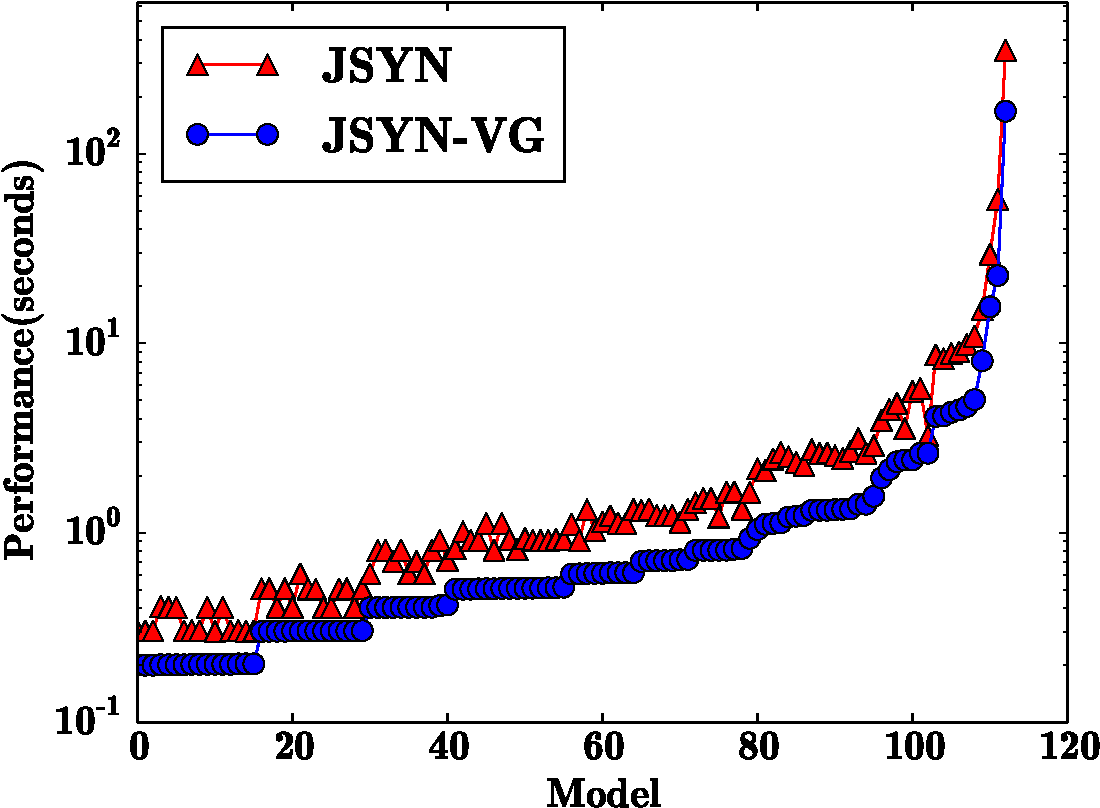
\includegraphics[width=2.15in]{overhead-crop}
\label{fg:performance}}
%\hspace{+6.5em}
\quad
\subfloat[Size of implementations]{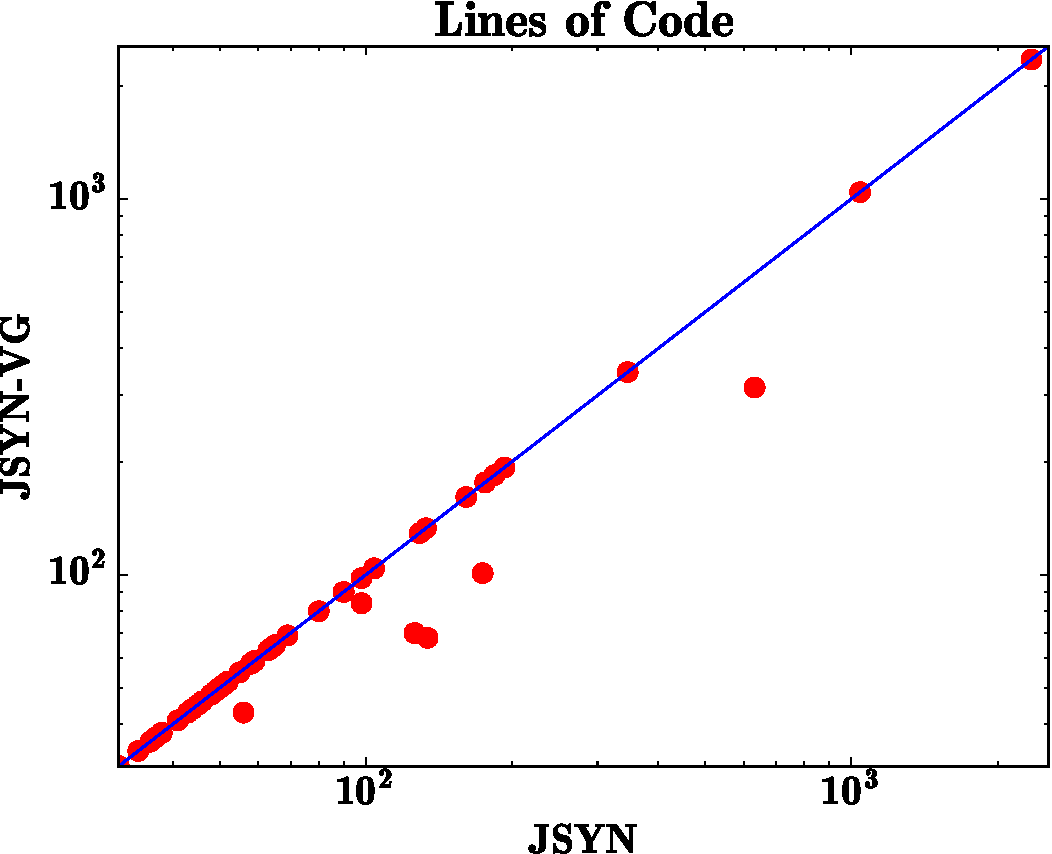
\includegraphics[width=2.15in]{loc-crop}
\label{fg:size}}
\vspace{-5pt}
\subfloat[Performance of implementations]{
\hspace{-1em}
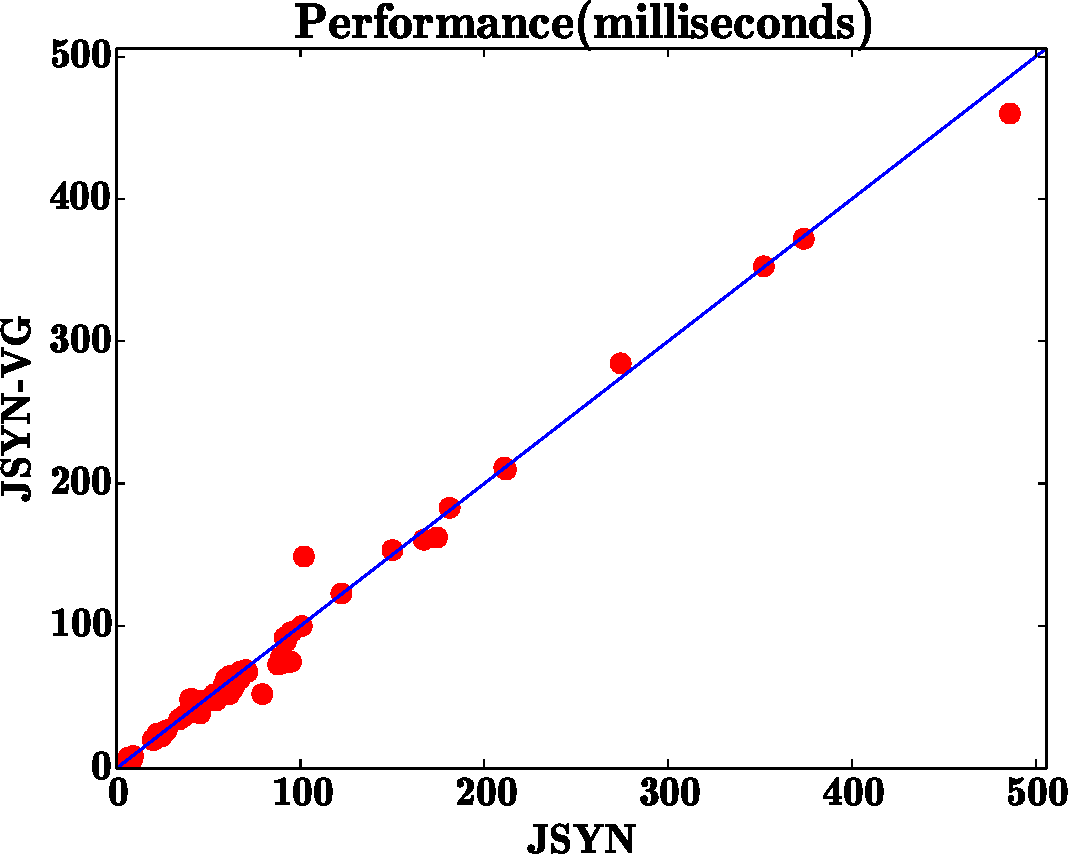
\includegraphics[width=2.15in]{performance-crop}
\label{fg:implperformance}}
\subfloat[Size of implementations after compaction]{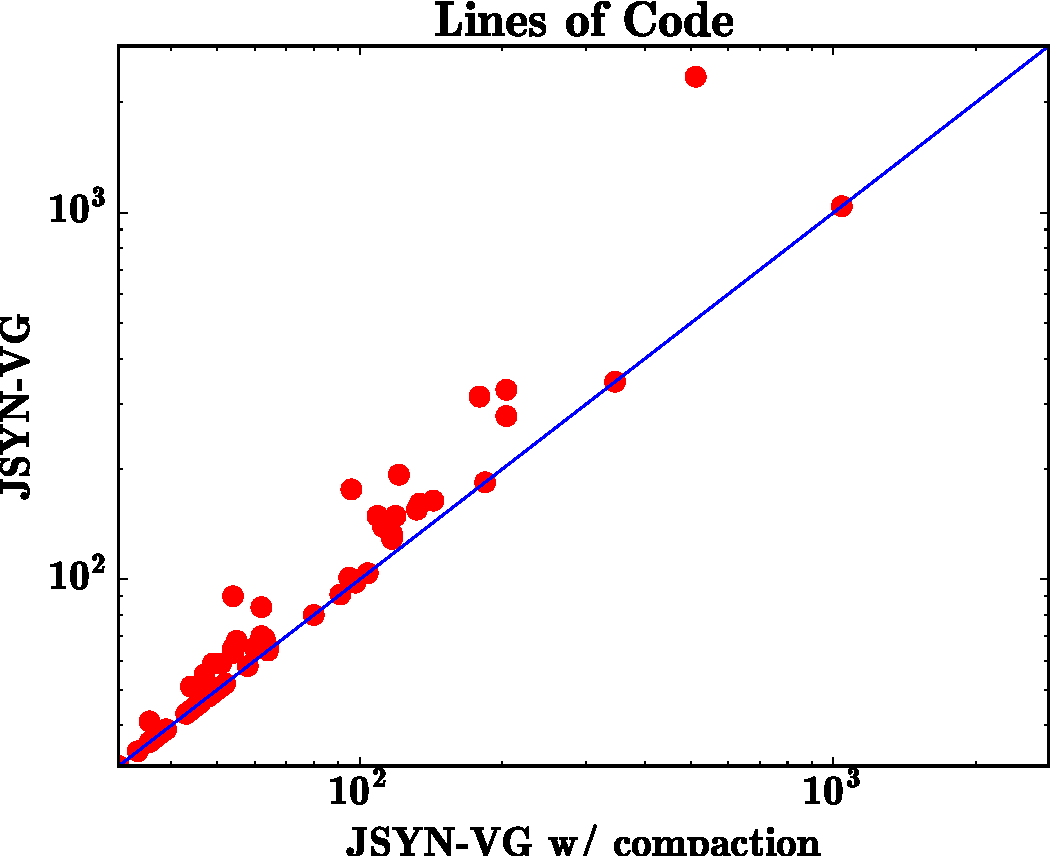
\includegraphics[width=2.15in]{loccompact-crop}
\label{fg:compactsize}}
\caption{Experimental results.}
\vspace{-5pt}
\label{fg:results}
\end{figure}


One last statistic that we tracked was the performance of the synthesized C
implementations in terms of execution time, which can be seen in Fig.~\ref{fg:implperformance}. The performance was computed as the mean of 1000000 iterations of executing each implementation using random input values.
 \iffalse
  For this purpose, we translated the
 generated witnesses from \jsyn and \jsynvg solutions using
 \smtlibtoc under the same set of options.
 \fi
 According to the figure as well as Table~\ref{tbl:stats}, the differences are minuscule on average.
\iffalse
while \jsyn implementations are faster, the difference is minuscule on average.
This small difference may occur due to the fact that \jsyn creates separate skolem functions for the initial evaluation
(when \%init is true)

and subsequent evaluations, whereas currently \jsynvg uses a single function for both cases, and as such requires the evaluation of richer expressions prior to choosing a proper reaction.
\fi

% The deciding factor in this context is the
% difference in complexity of the Model-Based Projections that get generated by
% \aeval using \jsyn and \jsynvg, with the latter versions containing richer
% expressions, mainly due to the refinement process.

\iffalse
Fig.~\ref{fg:results} does not cover the entirety of the
benchmark suite. From the original 124 problems, eleven of them cannot be
solved by \jsyn's $k$-inductive approach.
%\grigory{ideally, a summary of these observations should be pulled all the way towards the intro. Even more, It should probably be the main motivation of the entire work.}
Four of these files are variations of
the Cinderella-Stepmother game using different representations of the game, as well as two different values
for the bucket capacity (2 and 3). Using the variation in Fig.~\ref{fg:cind} as an input to \jsyn, we receive an ``unrealizable'' answer, with the counterexample shown
in Fig.~\ref{fg:cex}. Reading through the feedback provided by \jsyn, it is
apparent that the underlying SMT solver is incapable of choosing the correct
buckets to empty, leading eventually to a state where an overflow occurs for the
third bucket. As we already discussed though, a winning strategy exists for the
Cinderella game, as long as the bucket capacity \texttt{C} is between 1.5 and 3. This
provides an excellent demonstration of the inherent weakness of \jsyn
for determining unrealizability. \jsynvg's validity-guided approach,
is able to prove the realizability for these contracts, as
well as synthesize an implementation for each.

\begin{figure}[!t]
\centering
 \begin{Verbatim}[fontsize=\scriptsize]
	 ++++++++++++++++++++++++++++++++++++++++++++++++++++++++++
	      UNREALIZABLE || K = 6 || Time = 2.017s
	                 Step
	      variable      0    1      2      3      4      5
	      INPUTS
	      i1            0    0      0 0.416* 0.944* 0.666*
	      i2            1    0 0.083* 0.083*      0 0.055*
	      i3            0    1 0.305*    0.5 0.027* 0.194*
	      i4            0    0 0.611*      0      0 0.027*
	      i5            0    0      0      0 0.027* 0.055*
	
	      OUTPUTS
	      e             1    3      1      5      4      5
	
	      NODE OUTPUTS
	      guarantee   true true   true   true   true  false
	
	      NODE LOCALS
	      b1            0    0      0 0.416* 1.361* 0.666*
	      b2            0    0 0.083* 0.166* 0.166* 0.222*
	      b3            0    1 1.305* 1.805* 1.833* 2.027*
	      b4            0    0 0.611* 0.611*      0 0.027*
	      b5            0    0      0      0 0.027* 0.055*
	
	      * display value has been truncated
	 ++++++++++++++++++++++++++++++++++++++++++++++++++++++++++
 \end{Verbatim}
\vspace{-1.5em}
\caption{Spurious counterexample for Cinderella-Stepmother example using \jsyn}
\label{fg:cex}
\end{figure}
\fi
% \begin{table*}[!t]
% \centering
% \caption{Cinderella-Stepmother results}
% \label{tbl:cindtbl}
% \resizebox{0.7\textwidth}{!}{%
% \begin{tabular}{|c|c|c|c|c|c|}
% \hline
% \multirow{2}{*}{Game} & \multicolumn{3}{c|}{\jsynvg} & \multicolumn{2}{c|}{\textsc{ConSynth}~\cite{beyene2014constraint}} \\ \cline{2-6}
%  & \begin{tabular}[c]{@{}c@{}}Impl. Size\\ (LoC)\end{tabular} & \begin{tabular}[c]{@{}c@{}}Impl. Performance\\ (ms)\end{tabular} & Time & \begin{tabular}[c]{@{}c@{}}Time\\ (Z3)\end{tabular} & \begin{tabular}[c]{@{}c@{}}Time\\ (Barcelogic)\end{tabular} \\ \hline
% Cind (C = 3) & 204 & 128.09 & 4.5s & \multirow{2}{*}{3.2s} & \multirow{2}{*}{1.2s} \\ \cline{1-4}
% Cind2 (C = 3) & 2081 & 160.87 & 28.7s &  &  \\ \hline
% Cind (C = 2) & 202 & 133.04 & 4.7s & \multirow{2}{*}{1m52s} & \multirow{2}{*}{1m52s} \\ \cline{1-4}
% Cind2 (C = 2) & 1873 & 182.19 & 27.2s &  &  \\ \hline
% \end{tabular}}
% \end{table*}
% \begin{table*}[!t]
% \centering
% \caption{Cinderella-Stepmother results}
% \label{tbl:cindtbl}
% \begin{tabular}{|c|c|c|c|c|c|}
% \hline
%  & \multicolumn{3}{c|}{\jsynvg} & \multicolumn{2}{c|}{\textsc{ConSynth}~\cite{beyene2014constraint}} \\ \hline
%  & Implementation Size (LoC) & Implementation Performance (ms) & Time & Time (Z3) & Time (Barcelogic) \\ \hline
% Cinderella (C = 3) & 92 & 262.84 & 35s & \multirow{2}{*}{3.2s} & \multirow{2}{*}{1.2s} \\ \cline{1-4}
% Cinderella2 (C = 3) & 222 & 309.24 & 2m9s &  &  \\ \hline
% Cinderella (C = 2) & 102 & 196.57 & 24s & \multirow{2}{*}{1m52s} & \multirow{2}{*}{1m52s} \\ \cline{1-4}
% Cinderella2 (C = 2) & 272 & 230.16 & 2m9s &  &  \\ \hline
% \end{tabular}
% \end{table*}

Table~\ref{tbl:cindtbl} shows how \jsynvg performed on the four contracts describing the Cinderella-Stepmother game. We used two different interpretations for the game, and exercised both for the cases where the bucket capacity  \texttt{C} is equal to 2 and 3. Regarding the synthesized implementations, their size is analogous to the complexity of the program (Cinderella2 contains more local variables and a helper function to empty buckets). Despite this, the implementation performance remains the same across all implementations. Finally for reference, the table contains the results from the template-based approach followed in \textsc{Consynth}~\cite{beyene2014constraint}. From the results, it is apparent that providing templates yields better performance for the case of $C = 3$, but our approach overperforms \textsc{Consynth} when it comes to solving the harder case of $C = 2$. Finally, the original paper for \textsc{Consynth} also explores the synthesis of winning strategies for Stepmother using the liveness property that a bucket will eventually overflow. While \jkind does not natively support liveness properties, we successfully synthesized an implementation for Stepmother using a bounded notion of liveness with counters. We leave an evaluation of this category of specifications for future work.

Overall, \jsynvg's validity-guided approach provides significant advantages
over the $k$-inductive technique followed in \jsyn, and effectively expands
\jkind's solving capabilities regarding specification realizability. On top of that, it provides an efficient ``hands-off'' approach that is capable of solving complex games.
The most significant contribution, however, is the applicability of this approach, as it is not tied to a specific environment since it can be extended to support more
theories, as well as categories of specification. 

\section{Related Work}
\label{sec:related}

\iffalse
The alternative name to program synthesis is Church's problem, since the description of the problem was first described by Church in 1963~\cite{church1962logic}. Research in this field of program synthesis attributes began in the 1970s, when Manna and Waldinger~\cite{manna1971toward} first introduced a synthesis procedure using principles of theorem proving. Almost two decades later, Pnueliand Rosner~\cite{pnueli1989synthesis} first formally described the
implementability of reactive systems, considering first order logic formulas
that stem from temporal specifications. In the same work, they provided a
complete approach to synthesize finite-state implementations through the
construction of deterministic Rabin automata.

In the recent years, program synthesis has enjoyed a vast variety of
contributions under numerous contexts. Gulwani~\cite{gulwani2010dimensions}
presented an extended survey, hinting future research directions. Synthesis
algorithms have been proposed for simple LTL specification~\cite{Bohy12,Tini03}
subsets of it~\cite{Klein10,ehlers2010symbolic,cheng2016structural}, as well as under other temporal logics~\cite{monmege2016real,Hamza10}, such as SIS~\cite{Aziz95}.
Chatterjee and Henzinger~\cite{Chatterjee07} proposed a novel component-based approach using the notion of Assume-Guarantee contracts.
\fi
The work presented in this paper is closely related to approaches that attempt
to construct infinite-state implementations. Some focus on the continuous
interaction of the user with the underlying machinery, either through the use of
templates~\cite{srivastava2013template,beyene2014constraint}, or environments where the user attempts to guide the solver by choosing reactions from a collection of different
interpretations~\cite{ryzhyk2016developing}.
In contrast, our approach is completely automatic and does not require
human ingenuity to find a solution.
Most importantly, the user
does not need to be deeply familiar with the problem at hand.
\iffalse
 A ``hands-off'' approach has been proposed in the past by Katis \textit{et
al.}~\cite{gacek2015towards,katis2016towards,katis2016synthesis}. The work is
based on the concept of extracting collections of reactions that witness the satisfaction of a $k$-inductive proof on the contract's realizability.
In Section~\ref{sec:results} we were able to effectively show in practice how a
validity-guided approach significantly improves upon this work, by using a
fixpoint-generating technique rather than the principle of $k$-induction.
\fi

Iterative strengthening of candidate formulas is also used in abductive inference~\cite{dillig2013inductive}
 %Dillig \textit{et al.} showed how abduction can be used
of loop invariants.
Their approach generates candidate invariants as maximum universal subsets (MUS) of quantifier-free formulas of the form $\phi \Rightarrow \psi$.
%   via a refinement process that generates candidate invariants in the form of maximum universal subsets (MUS).
While a MUS may be sufficient to prove validity, it may also mislead the invariant search, so the authors use a backtracking procedure that discovers new subsets while avoiding spurious results. By comparison, in our approach the regions of validity are maximal and therefore backtracking is not required.  More importantly, reactive synthesis requires mixed-quantifier formulas, and it requires that inputs are unconstrained (other than by the contract assumptions), so substantial modifications to the MUS algorithm would be necessary to apply the approach of~\cite{dillig2013inductive} for reactive synthesis.  %In our work, the ability to generate precise regions of validity lead to a very simple refinement process that is solely based on the input variables being existentially quantified.

The concept of synthesizing implementations by discovering fixpoints was mostly
inspired by the IC3 / PDR~\cite{bradley2011sat,een2011efficient}, which was first introduced
in the context of verification. Work from Cimatti \textit{et al.} effectively
applied this idea for the parameter synthesis in the
\textsc{HyComp} model checker~\cite{DBLP:conf/fmcad/CimattiGMT13, cimatti2015hycomp}.
Discovering fixpoints to synthesize reactive designs was first
extensively covered by Piterman \textit{et al.}~\cite{piterman2006synthesis}
who proved that the problem can be solved in cubic time for the class of GR(1) specifications.
The algorithm requires the discovery of least fixpoints for the state variables,
each one covering a greatest fixpoint of the input variables. If the specification
is realizable, the entirety of the input space is covered by the greatest fixpoints.
In contrast, our approach computes a single greatest fixpoint over the system's outputs and avoids the partitioning of the input space.  As the tools use different notations and support different logical fragments, practical comparisons are not straightforward, and thus are left for the future.

More recently, Preiner \textit{et al}. presented work on model synthesis~\cite{preiner2017counterexample}, %that constructs candidate witnesses constructed and their validity is checked with respect to the specification. Internally,
that employs a counterexample-guided refinement process~\cite{reynolds2015counterexample}
to construct and check candidate models.
Internally, it relies on enumerative learning, a syntax-based technique that enumerates expressions, checks their validity against
ground test cases, and proceeds to generalize the expressions by constructing larger ones.
In contrast, our approach is syntax-insensitive in terms of generating regions of validity.
\iffalse
On top of that, CEGMS has only been tested against the theory of Boolean Vectors (BV, and BV$_{LNIRA}$), while \jsynvg supports the mixed theories of linear integer and real arithmetic.
\fi
In general, enumeration techniques such as the one used in \textsc{ConSynth}'s underlying E-HSF engine~\cite{beyene2014constraint} is not an optimal strategy for our class of problems, since the witnesses constructed for the most complex contracts are described by nested if-then-else expressions of depth (i.e. number of branches) 10-20, a point at which space explosion is difficult to handle since the number of candidate solutions is large.

\section{Conclusion and Future Work}
\label{sec:conclusion}

% \subsection{Summary}

We presented a novel and elegant approach towards the synthesis
of reactive systems, using only the knowledge provided by the
system specification expressed in infinite theories.
\iffalse
 The approach is
directly inspired from previous work on Property Directed Reachability, with the objective being the construction of inductive
invariants that can be used as a proof to the specification's realizability.
\fi
The main goal is to converge to a fixpoint by iteratively blocking subsets of
unsafe states from the problem space. This is achieved through the continuous
extraction of regions of validity which hint towards subsets of states that
lead to a candidate implementation.

This is the first complete attempt, to the best of our knowledge, on handling
valid subsets of a $\forall\exists$-formula to construct a greatest fixpoint on specifications expressed using infinite theories. We were able to
prove its effectiveness in practice, by comparing it to an already existing
approach that focuses on constructing $k$-inductive proofs of realizability. We showed how the new algorithm performs better than the $k$-inductive approach, both in terms of performance as well as the soundness of results. In the future, we would like to extend the applicability of this algorithm to other areas in formal verification, such as invariant generation. Another interesting goal is to make the proposed benchmark collection available to competitions such as SYNTCOMP, by establishing a formal extension for the TLSF format to support infinite-state problems~\cite{DBLP:journals/corr/Jacobs016}. Finally, a particularly interesting challenge is that of mapping infinite theories to finite counterparts, enabling the synthesis of secure and safe implementations.

\iffalse
\subsection{Future Work}
Research in the area of program synthesis, and particularly the work presented in this paper, is rich with challenges and promising directions. We enlist the most important challenges that we would like to address as part of future work.

\textbf{Optimizations and Machine-Checked Proofs}. The most interesting question is how we can possibly improve \jsynvg's
speed of convergence. Not excluding techniques such as counterexample-guided
refinement and predicate abstraction~\cite{walker2014predicate}, a potential
improvement could be achieved through the use of a more compact transition
relation. Regarding the synthesized implementations, an interesting subproblem to examine the potential benefits of a subprocess that provides collections of equivalent implementations, rather than
a single witness. There are several promising concepts that can lead to further implementation optimization, such as the use of Inductive Validity Cores~\cite{Ghass16}, which can be potenitally used to identify the core elements in a synthesized implementation that lead to the satisfaction of the specification. Using only the core elements, we can effectively reduce the size of the implementations, and improve their performance. Another interesting direction in pursuing compact implementations exploited is to examine the effects of recent work in witness abstractions~\cite{jakobs2017compact}. Finally, a short-term goal is the development of machine-checked
proofs regarding the soundness of the fixpoint generation process, as well as the realizability results.

\iffalse
\textbf{Test case generation}. \aeval's effectiveness in providing witnesses to the
satisfiability of $\forall\exists$-formulas can be also exploited in terms of the
tool providing concrete counterexamples to a subset of unrealizable contracts that relate to formula $\phi' \gets \forall s. \ (F(s) \Rightarrow \exists i. A(s,i) \land \lnot Q(s,i))'$ being valid (Algorithm~\ref{alg:synthesis}, Line 16).
In this particular case, if $\phi'$ is a valid formula, it is possible a witness that can be essentially used as a test case to demonstrate the specification's unrealizability. The witness contains
certain assignments to input variables, for which the condition of viability does not hold, for any state. In conjunction with the potential capabilities of generating collections of equivalent implementations, this problem may lead to the creation of an elegant process that constructs test suites against the contract's realizability. Such a test suite can then be used as a complementary collection to testing procedures that take place towards the end of the system's development.
\fi
\textbf{Mapping infinite theories to finite representations}. A particularly challenging topic of research, is how we can transition from implementations that use
infinite types through SMT, to equivalent ones using finite representations, without violating the specification. The SMT community has already kickstarted a project towards achieving this, through a recently introduced theory on Floating-Point Arithmetic~\cite{brain2015automatable}. The problem is particularly interesting for the cases where the high-end user has to define secure contracts that contain properties for memory allocation, representation of floats, and overflow handling.
\fi 
%\input{artifact}

%\subsubsection*{\textbf{Acknowledgments}}
%This work was funded by DARPA and AFRL under contract FA8750-12-9-0179 (Secure
% Mathematically-Assured Composition of Control Models), and by NASA under contract NNA13AA21C (Compositional Verification of Flight Critical Systems), and by NSF under grant CNS-1035715 (Assuring the safety, security, and reliability of medical device cyber physical systems).
% \IEEEtriggeratref{25}
\bibliography{document}
\bibliographystyle{splncs03}
\end{document}
